\section{Μοντελοποίηση Κλάσεων εκτίμησης πόζας}

Για την εφαρμογή \textsl{Exercisor} χρησιμοποιήθηκε η βιβλιοθήκη Kivy, ακρογωνιαίος λίθος της οποίας είναι το μοντέλο Model-View-Controller, όπως περιγράφηκε στην ενότητα \ref{sec:mvc}. Επεξηγηματικά, το επίπεδο \textsl{View} επιτυγχάνεται με το Kivy χρησιμοποιώντας την γλώσσα \texttt{KV}\footnote{\href{https://kivy.org/doc/stable/guide/lang.html}{https://kivy.org/doc/stable/guide/lang.html}}, σε ειδικά αρχεία κατάληξης \texttt{.kv}, τα οποία χρησιμοποιούνται για να καθορίσουν τα γραφικά στοιχεία, την εμφάνιση τους και την διάταξή τους στην οθόνη. Ταυτόχρονα, οι κλάσεις ορισμένες με την γλώσσα \texttt{KV} είναι συνδεδεμένες προαιρετικά με τον αντίστοιχο ορισμό τους στην γλώσσα Python, η λογική του οποίου υλοποιεί το επίπεδο \textsl{Controller}.

Στο παρών κεφάλαιο θα αναλυθούν οι κλάσεις και οι σχέσεις μεταξύ τους με την γλώσσα UML, αναφέροντας σχεδιαστικά πρότυπα που χρησιμοποιήθηκαν. Σημειώνεται ότι δεν θα επεκταθούμε στον τρόπο λειτουργίας των μοντέλων μηχανικής μάθησης HMR και SMPL, καθώς από την μία ο κώδικας δεν αναπτύχθηκε από εμάς, και από την άλλη περιγράφεται εκτενώς η λειτουργία τους στα κεφάλαια \ref{sec:hmr} και \ref{sec:smpl} αντίστοιχα. Επίσης, δεν θα σχολιάσουμε τον τρόπο παραγωγής γραφικών με την γλώσσα \textsl{KV} παρά μόνο τους αντίστοιχους ελεγκτές που χρήζουν σχολιασμό.

\newpage
\subsection{ExercisorScreen}

\begin{figure}[h]
	\centering
	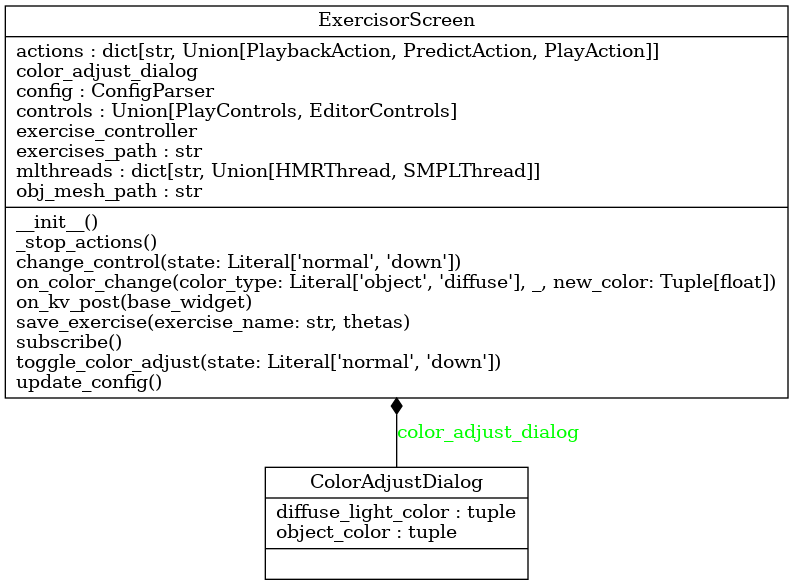
\includegraphics[scale=0.4]{images/chapter5/exercisor_uml.png}
	\caption{UML διάγραμμα της κλάσης \texttt{ExercisorScreen}}
	\label{fig:exercisor_uml}
\end{figure}

\noindent\textbf{Περιγραφή Κλάσης}
Η κλάση αυτή κληρονομεί από την κλάση ScreenManager\footnote{ \href{https://kivy.org/doc/stable/api-kivy.uix.screenmanager.html\#kivy.uix.screenmanager.ScreenManager}{https://kivy.org/doc/stable/api-kivy.uix.screenmanager.html\#kivy.uix.screenmanager.ScreenManager}} και είναι η βασική κλάση του \textsl{Exercisor}.

Κατά την αρχικοποίηση της, στην μέθοδο \texttt{\_\_init\_\_} φορτώνονται τα αρχεία \texttt{.kv} και με το πέρας της διαδικασίας εκτελείται η συνάρτηση \texttt{on\_kv\_post()}. Τότε, γίνεται η αρχικοποίηση του ελεγκτή λειτουργίας \textsl{παιχνιδιού}, \texttt{controls}, κλάση τύπου \texttt{AbstractControls} \ref{sec:abstract_controls}, των διαθέσιμων ενεργειών, \texttt{actions} κλάσεις τύπου \texttt{AbstractAction} \ref{sec:abstract_actions}, οι οποίες με την σειρά τους αρχικοποιούν τα threads των μοντέλων βαθιάς μηχανικής μάθησης, \texttt{mlthreads} κλάσεις τύπου \texttt{MLThread} \ref{sec:ml_threads}. Επιπλέον, αρχικοποιείται ο \texttt{exercise\_controller}, κλάση τύπου \texttt{ExerciseController} \ref{sec:exercise_controller}, ο οποίος είναι ο ελεγκτής των διαθέσιμων ασκήσεων. Ένα εποπτικό UML διάγραμμα της αρχιτεκτονικής φαίνεται στο Σχήμα \ref{fig:exercisor_relations}.

\begin{figure}[h]
	\centering
	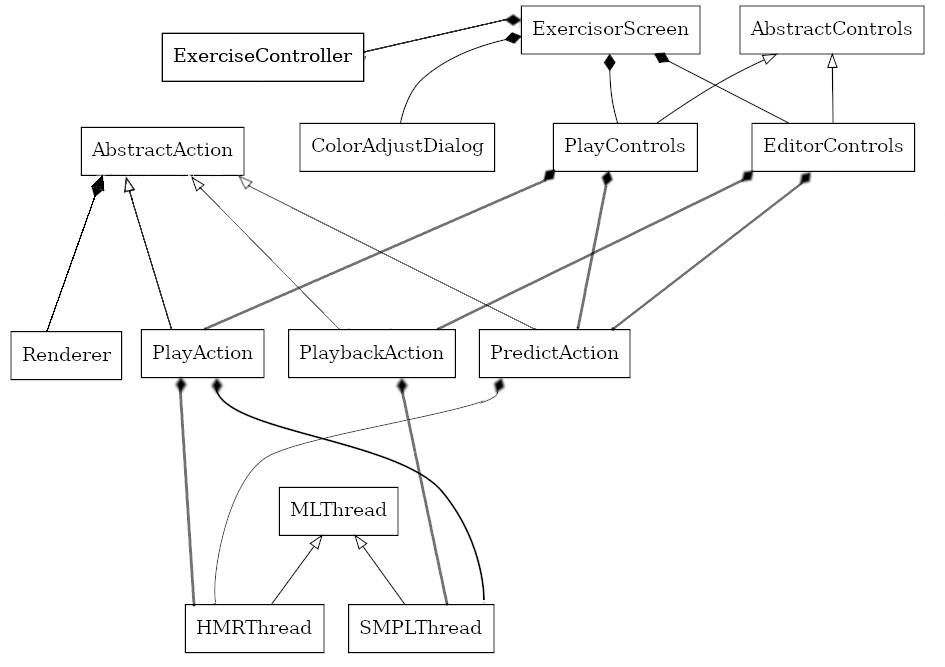
\includegraphics[scale=0.4]{images/chapter5/overview_exercisor_screen.png}
	\caption{Εποπτικό UML διάγραμμα  σχέσεων του \texttt{ExercisorScreen}.}
	\label{fig:exercisor_relations}
\end{figure}

\noindent\textbf{Χαρακτηριστικά κλάσης}\footnote{Σημειώνεται ότι στις επεξηγήσεις των χαρακτηριστικών και των μεθόδων παραλείπονται αυτές που έχουν ήδη αναφερθεί ή που είναι προφανής η χρήση τους. Επίσης, όταν παραλείπεται μέθοδος δόμησης \textsl{\_\_init()\_\_} που παίρνει ορίσματα, θεωρείται ότι το μόνο που κάνει είναι να αναθέσει τα αντίστοιχα ορίσματα σε χαρακτηριστικά της κλάσης.}
\begin{itemize}
	\item \texttt{config}: Μεταβλητή τύπου kivy.properties.ConfigParserProperty\footnote{\href{https://kivy.org/doc/stable/api-kivy.properties.html\#kivy.properties.ConfigParserProperty}{https://kivy.org/doc/stable/api-kivy.properties.html\#kivy.properties.ConfigParserProperty}} που επιτρέπει την αλλαγή του path των προ-εκπαιδευμένων μοντέλων, του φακέλου με τα δεδομένα ασκήσεων και του αρχικού φακέλου με τα βίντεο για είσοδο ασκήσεων αναφοράς.
	\item \texttt{exercises\_path}: To path του φακέλου όπου βρίσκονται αποθηκευμένα τα δεδομένα ασκήσεων αναφοράς.
	\item \texttt{object\_mesh\_path}: To path όπου βρίσκεται ένα αρχείο πλέγματος κατάληξης \texttt{.obj} που μπορεί να χρησιμοποιηθεί για αποσφαλμάτωση.
\end{itemize}

\noindent\textbf{Μέθοδοι Κλάσης}
\begin{itemize}
	\item \texttt{change\_control(state)}: Αλλάζει τα κουμπιά στο κάτω μέρος της οθόνης από λειτουργία \texttt{παιχνιδιού} σε λειτουργία \texttt{επιμελητή} και ανάποδα, ανάλογα με την τιμή του \texttt{state}, Σχήμα \ref{fig:basic_screens_ui}. 
	\item \texttt{toggle\_color\_adjust(state)}: Εμφανίζει ή σβήνει το γραφικό της κλάσης \texttt{ColorAdjustDialog}, ανάλογα με την τιμή του \texttt{state}, Σχήμα \ref{fig:play_screen}. Μέσω αυτού του στοιχείου, εκτελείται η μέθοδος \texttt{on\_color\_change(color\_type, new\_color)} η οποία θέτει το RGB χρώμα \texttt{new\_color} στο χρώμα του \textsl{ambient} φωτισμού ή του χρώματος των απεικονιζόμενων πλεγμάτων ανάλογα με το \texttt{color\_type}.
	\item \texttt{subscribe()}: Συνάρτηση η οποία εκθέτει στον Controller τις εντολές που δέχεται το Widget και ποιες συναρτήσεις θα εκτελεστούν.
	\item \texttt{update\_config()}: Συνάρτηση η οποία διαβάζει τις ρυθμίσεις και ανανεώνει κατάλληλα τις μεταβλητές της κλάσης.
	\item \texttt{save\_exercise(exercise\_name,thetas)}: Αποθηκεύει με όνομα \texttt{exercise\_name} τα δεδομένα άσκησης αναφοράς \texttt{thetas} που είναι ένας πίνακας $N \times 82$, όπου N ο αριθμός των καρέ του βίντεο και 82 οι παράμετροι του μοντέλου SMPL.
\end{itemize}

\begin{figure}[h]
	\centering
	\begin{subfigure}[h]{0.45\textwidth}
		\centering
		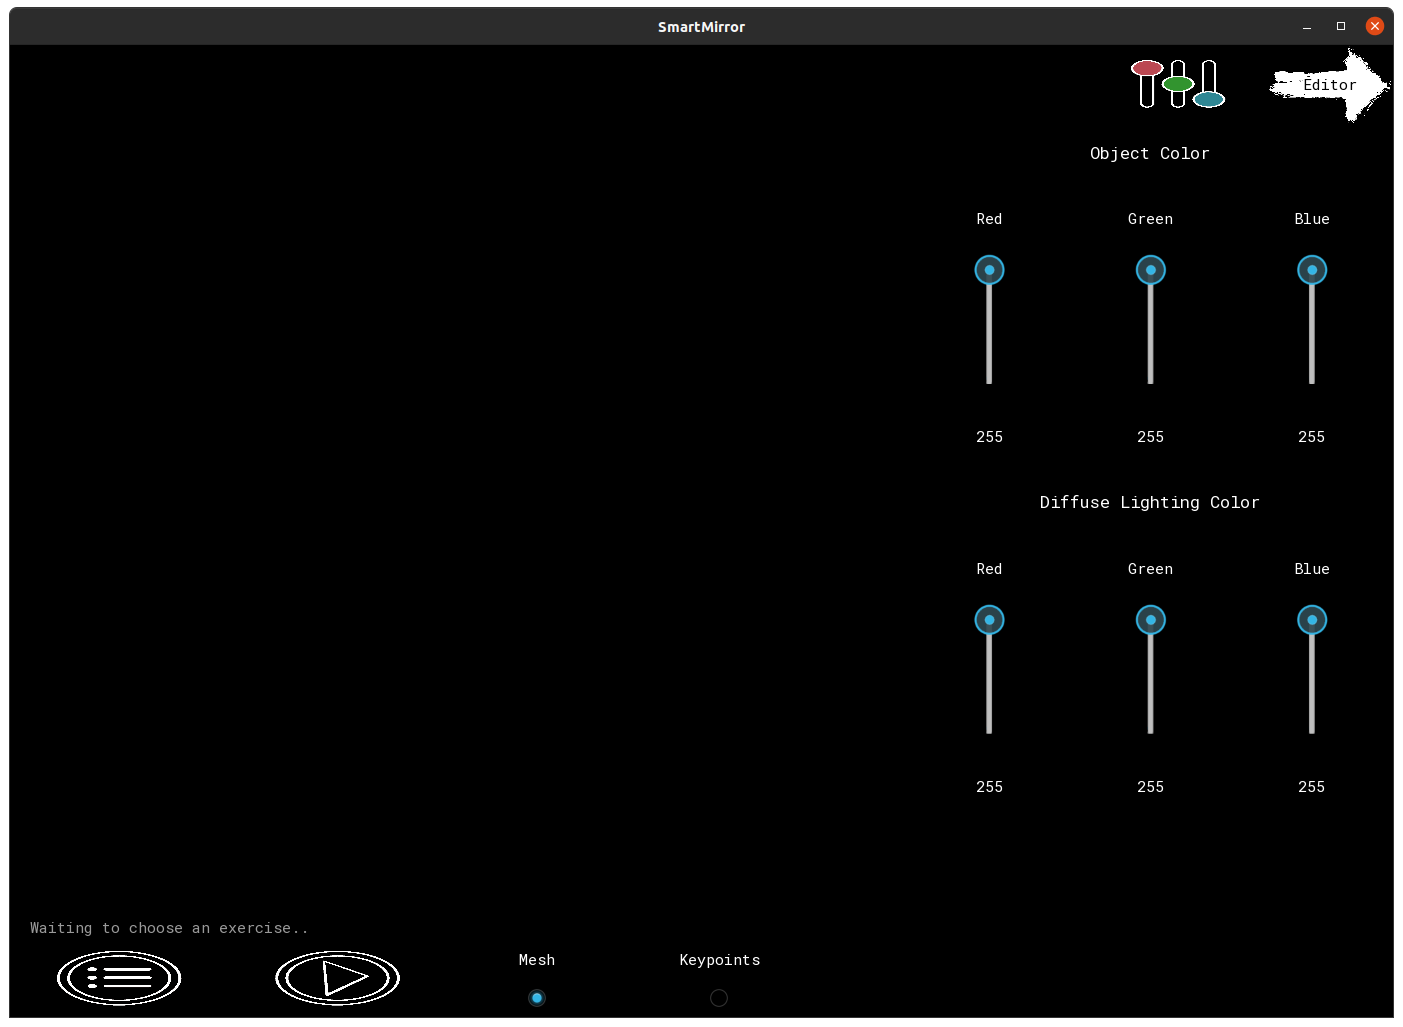
\includegraphics[width=\textwidth]{images/chapter5/play_screen.png}
		\caption[H λειτουργία \textsl{παιχνιδιού}]{H λειτουργία \textsl{παιχνιδιού}. Κάτω φαίνεται το widget \texttt{PlayControls} ενώ στα δεξιά φαίνεται το widget \texttt{ColorAdjustDialog}.}
		\label{fig:play_screen}
	\end{subfigure}
	\hfill
	\begin{subfigure}[h]{0.45\textwidth}
		\centering
		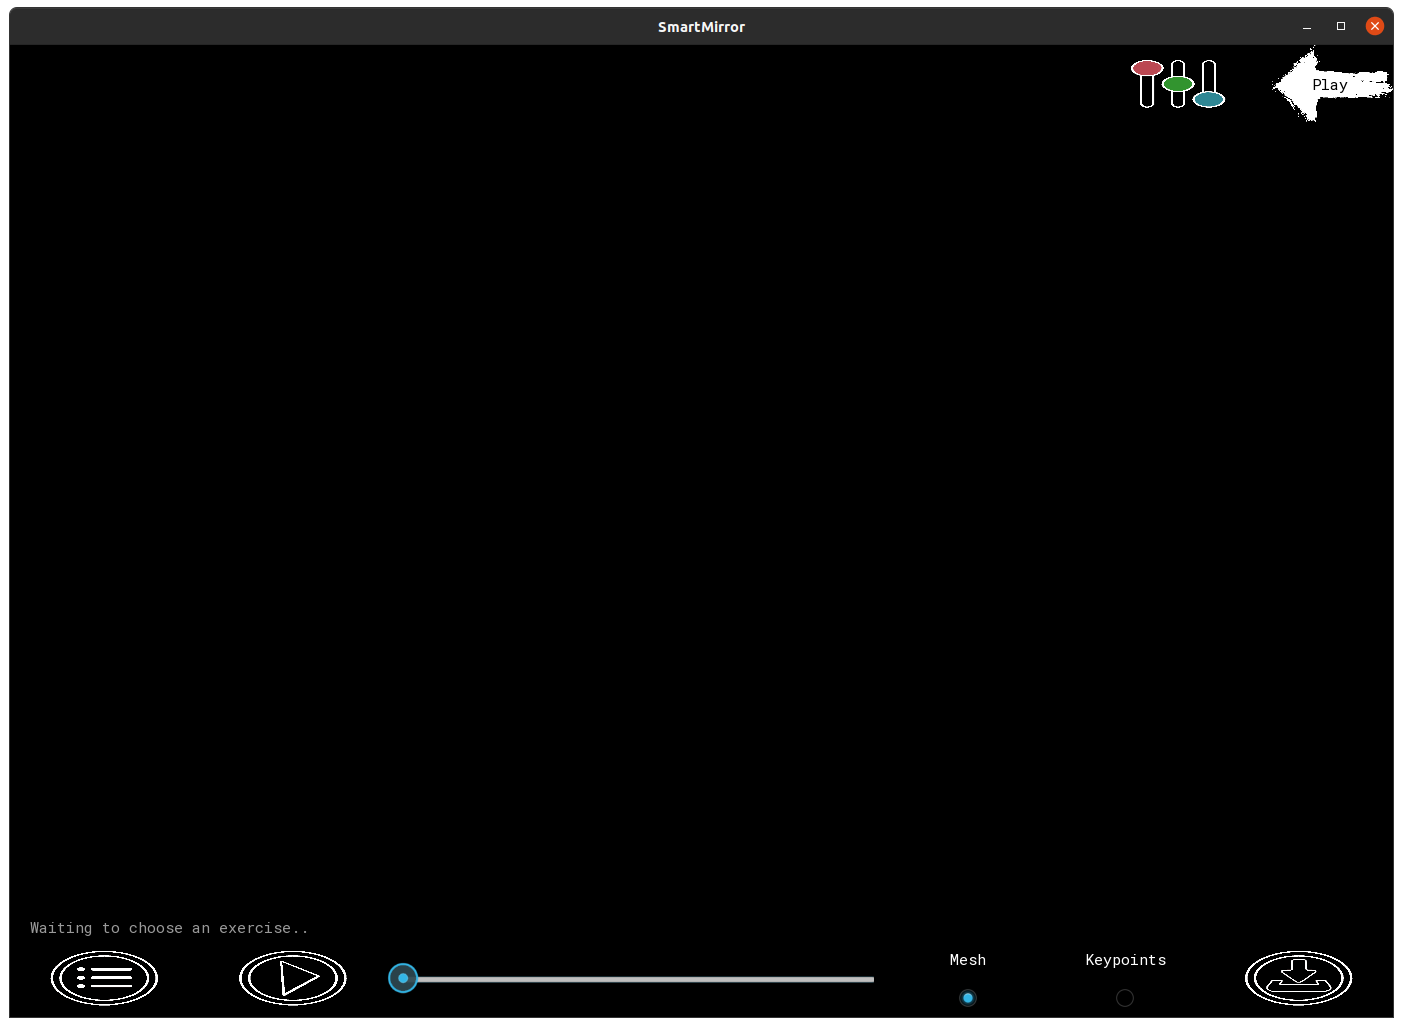
\includegraphics[width=\textwidth]{images/chapter5/editor_screen.png}
		\caption[H λειτουργία \textsl{επιμελητή}]{H λειτουργία \textsl{επιμελητή}. Κάτω φαίνεται το widget \texttt{EditorControls}.}
		\label{fig:editor_screen}
	\end{subfigure}
	\caption{Οι βασικές λειτουργίες του \textsl{Exercisor}}
	\label{fig:basic_screens_ui}
\end{figure}



\subsection{ExerciseController}
\label{sec:exercise_controller}
\begin{figure}[H]
	\centering
	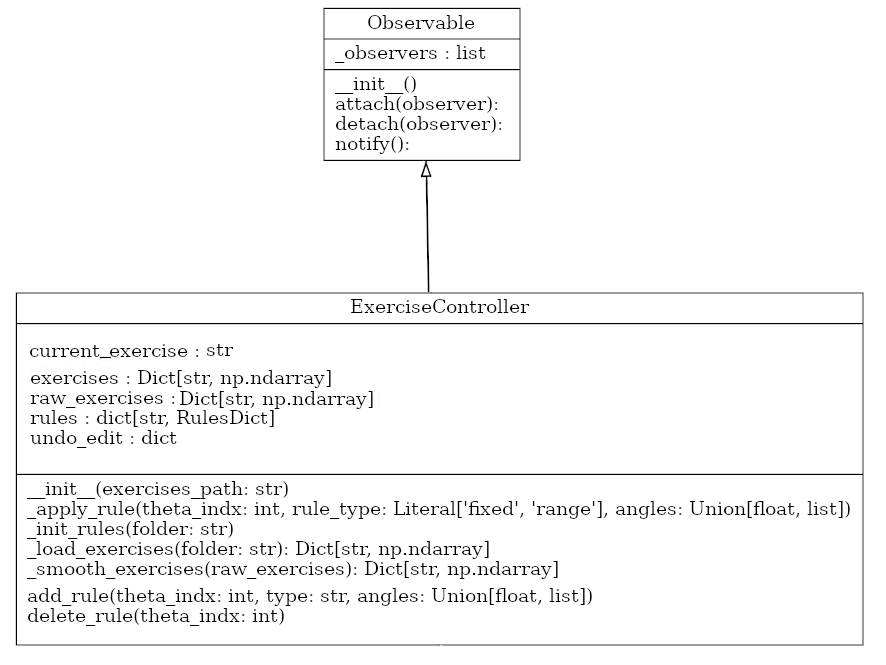
\includegraphics[scale=0.4]{images/chapter5/exercise_controller.png}
	\caption{UML διάγραμμα της κλάσης \texttt{ExerciseController}}
	\label{fig:controls}
\end{figure}

\noindent\textbf{Περιγραφή Κλάσης}
Η κλάση αυτή είναι υπεύθυνη για την διαχείριση των διαθέσιμων ασκήσεων και την επεξεργασία τους. 

Κληρονομεί από την κλάση \texttt{Observable} η οποία παρέχει μεθόδους για την υλοποίηση του σχεδιαστικού προτύπου \textsl{Observer Pattern}\footnote{\href{https://en.wikipedia.org/wiki/Observer\_pattern}{https://en.wikipedia.org/wiki/Observer\_pattern}}.
Αναλυτικότερα, αντικείμενα που ενδιαφέρονται για τις διαθέσιμες ασκήσεις πρέπει να υλοποιούν μία μέθοδο \texttt{update()} και να καλούνε την μέθοδο \texttt{attach} με όρισμα τον εαυτό τους, η οποία τις βάζει στην λίστα \texttt{\_observers}. Έτσι, όταν οι ασκήσεις, \texttt{exercises}, ανανεώνονται, καλείται η μέθοδος \texttt{notify()} η οποία καλεί την \texttt{update()} όλων των εγγεγραμμένων αντικειμένων. Αναφορικά, τα αντικείμενα που εγγράφονται στις ασκήσεις είναι οι ελεγκτές τύπου \texttt{PlayControls} και \texttt{EditorControls}.

\noindent\textbf{Χαρακτηριστικά κλάσης}
\begin{itemize}
	\item \texttt{current\_exercise}: Το όνομα της τωρινής άσκησης. Όλες οι επεξεργασίες γίνονται πάνω στην τωρινή άσκηση.
	\item \texttt{exercises}: Ένα dictionary με key το όνομα της άσκησης και value έναν πίνακα $Ν \times 82$, όπου N ο αριθμός των καρέ της άσκησης και 82 οι παράμετροι SMPL. Τα δεδομένα αυτών των ασκήσεων είναι μετά από την οποιαδήποτε επεξεργασία.
	\item \texttt{raw\_exercises}: Οι ασκήσεις όπως αναφέρθηκε παραπάνω αλλά με τα δεδομένα έτσι όπως είναι αποθηκευμένα, πριν από επεξεργασία.
	\item \texttt{rules}: Περιλαμβάνει κανόνες επεξεργασίας των ασκήσεων. Τα keys είναι το όνομα της άσκησης, ενώ το \texttt{RulesDict} είναι ένα dictionary με key έναν δείκτη που ορίζει μία παράμετρο από τις 82 και values ένα tuple της μορφής (rule\_type, angles), όπου καθορίζεται αν ο κανόνας επεξεργασίας είναι \textsl{fixed} ή \textsl{range} και οι σταθερές γωνίες περιορισμού.
	\item \texttt{undo\_edit}: Dictionary αντίστοιχης μορφής με το \texttt{rules} που κρατάει όμως τις παραμέτρους SMPL για κάθε καρέ πριν την επεξεργασία.
\end{itemize}

\noindent\textbf{Μέθοδοι Κλάσης}
\begin{itemize}
	\item \texttt{\_\_init\_\_(exercises\_path)}: Διαβάζει τα δεδομένα των αποθηκευμένων ασκήσεων από το path \texttt{exercise\_path} με χρήση της \texttt{\_load\_exercises}, αρχικοποιεί του κανόνες με την \texttt{\_init\_rules()} και εφαρμόζει ομαλοποίηση με την \texttt{\_smooth\_exercises}. 
	\item \texttt{\_apply\_rule(theta\_indx, rule\_type, angles)}: Επεξεργάζεται την παράμετρο με δείκτη \texttt{theta\_indx} της τωρινής άσκησης, εφαρμόζοντας έναν κανόνα τύπου \textsl{fixed} ή \textsl{range} περιορίζοντας τις γωνίες που μπορεί να πάρει.
	\item \texttt{\_init\_rules(folder)}: Αρχικοποιεί το dictionary με τους κανόνες επεξεργασίας με βάση τους αποθηκευμένους.
	\item \texttt{\_load\_exercises(folder)}: Διαβάζει τον φάκελο με τις αποθηκευμένες ασκήσεις τις μετατρέπει σε ένα dictionary και το επιστρέφει.
	\item \texttt{\_smooth\_exercises(self, raw\_exercises)}: Εφαρμόζει έναν αλγόριθμο κινούμενου μέσου\footnote{\href{https://en.wikipedia.org/wiki/Moving\_average}{https://en.wikipedia.org/wiki/Moving\_average}} με παράθυρο 10 καρέ στις παραμέτρους SMPL για κάθε άσκηση. Αυτό γίνεται για να ομαλοποιηθούν οι προβλέψεις από καρέ σε καρέ και να μην 'τρέμει' η απεικόνιση του ανθρώπινου πλέγματος.
	\item \texttt{add\_rule(theta\_indx, type, angles)}: Βάζει τον κανόνα στα \texttt{rules} και καλεί την \texttt{\_apply\_rule}.
	\item \texttt{delete\_rule(theta\_indx)}: Αφαιρεί τον κανόνα από τα \texttt{rules} και επαναφέρει τις παραμέτρους ανά καρέ από το \texttt{undo\_edit}.
\end{itemize}


\subsection{Controls}
\label{sec:abstract_controls}

\begin{figure}[H]
	\centering
	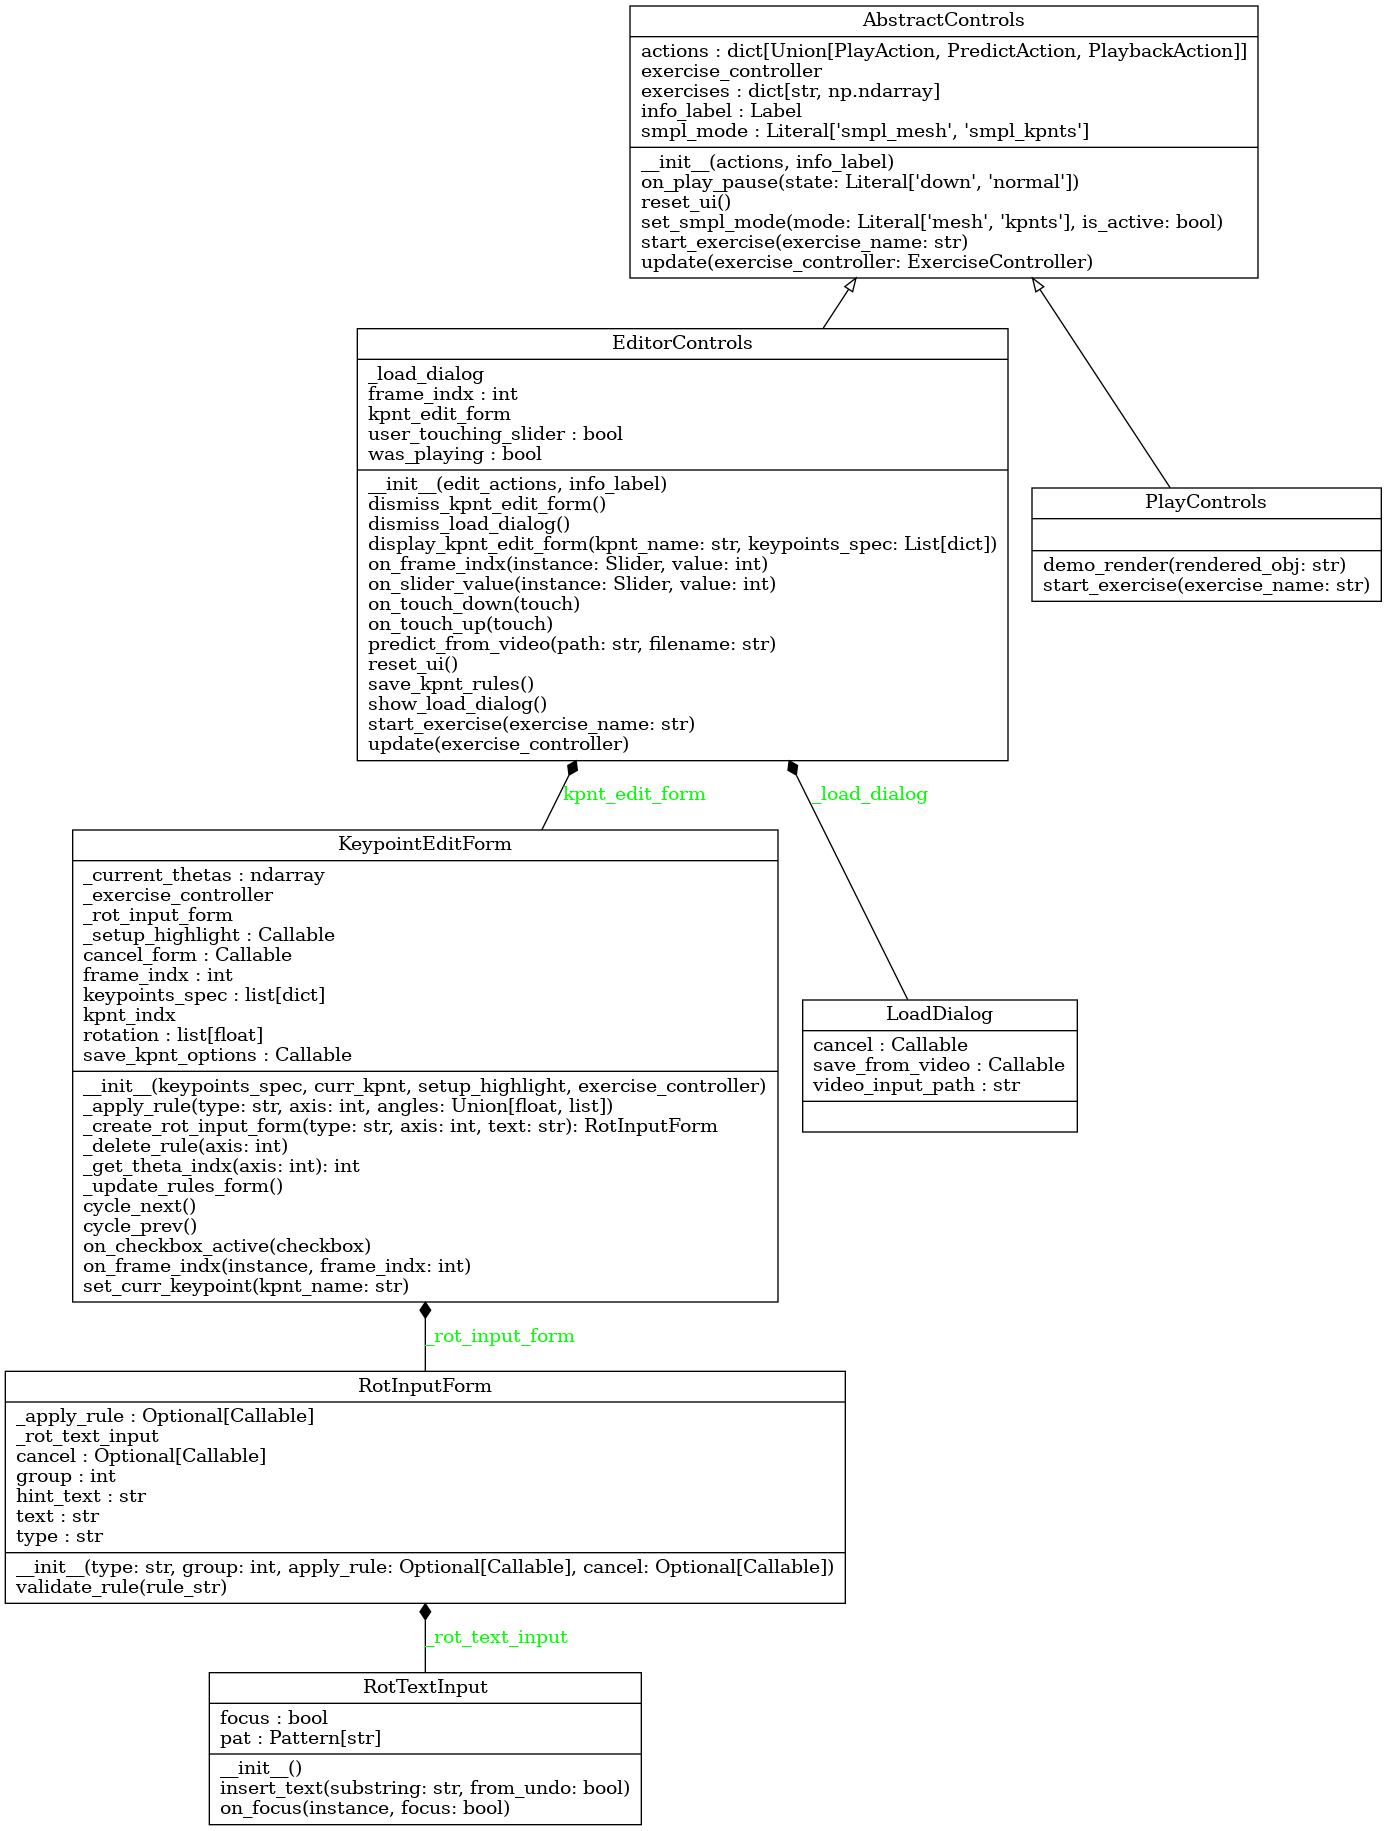
\includegraphics[scale=0.26]{images/chapter5/controls.png}
	\caption{UML διάγραμμα των κλάσεων τύπου \texttt{AbstractControls} και των σχέσεων τους.}
	\label{fig:controls}
\end{figure}

\noindent\textbf{Περιγραφή Κλάσεων}
Οι κλάσεις αυτές είναι υπεύθυνες για την διαχείριση των διαθέσιμων ενεργειών, \texttt{actions}, στην εκάστοτε λειτουργία. Όπως φαίνεται στο Σχήμα \ref{fig:exercisor_relations}, η κλάση \texttt{PlayControls} διαχειρίζεται τα actions τύπου \texttt{PlayAction} και \texttt{PredictAction}, ενώ η \texttt{EditorControls} τα actions \texttt{PlaybackAction} και \texttt{PredictAction}. Η γραφική τους απεικόνιση φαίνεται στο Σχήμα \ref{fig:controls_ui}.\footnote{Η εφαρμογή Exercisor, όπως αναφέρθηκε εξάγει τις εντολές αναγκαίες για την έναρξη του παιχνιδιού. Πιο περίπλοκες ενέργειες όμως, όπως οι λειτουργίες του \textsl{επιμελητή}, απαιτούν την χρήση ποντικιού και πληκτρολογίου. Ιδανικά οι λειτουργίες του \textsl{επιμελητή} δεν πρέπει να γίνονται πάνω στον καθρέφτη αλλά σε εξωτερικό σύστημα.}

\begin{figure}[h]
	\centering
	\begin{subfigure}[h]{0.45\textwidth}
		\centering
		
\includegraphics[width=\textwidth]{images/chapter5/play_controls.png}
		\caption{Τα controls του \textsl{παιχνιδιού}, \texttt{PlayControls}.}
		\label{fig:play_controls}
	\end{subfigure}
	\hfill
	\begin{subfigure}[h]{0.45\textwidth}
		\centering
		
\includegraphics[width=\textwidth]{images/chapter5/editor_controls.png}
		\caption{Τα controls του \textsl{επιμελητή}, \texttt{EditorControls}}
		\label{fig:editor_controls}
	\end{subfigure}
	\caption{Η γραφική αναπαράσταση των κλάσεων τύπου \texttt{AbstractControls}.}
	\label{fig:controls_ui}
\end{figure}

\noindent\textbf{Χαρακτηριστικά κλάσης}
Τα χαρακτηριστικά \texttt{actions}, \texttt{exercise\_controller} και \texttt{exercises} έχουν ήδη σχολιαστεί.
\begin{itemize}
	\item \texttt{info\_label}: Το widget κειμένου πληροφορίας που φαίνεται πάνω από τα κουμπιά στα αριστερά της οθόνης στο Σχήμα \ref{fig:controls_ui}.
	\item \texttt{smpl\_mode}: Ο τρόπος προβολής του ανθρώπου. Μπορεί να είναι είτε 'smpl\_mesh' είτε 'smpl\_kpnts' για την απεικόνιση του πλέγματος ή του σκελετού αντίστοιχα, όπως φαίνεται στο Σχήμα \ref{fig:render_options}.
\end{itemize}

\begin{figure}[h]
	\centering
	\begin{subfigure}[h]{0.45\textwidth}
		\centering
		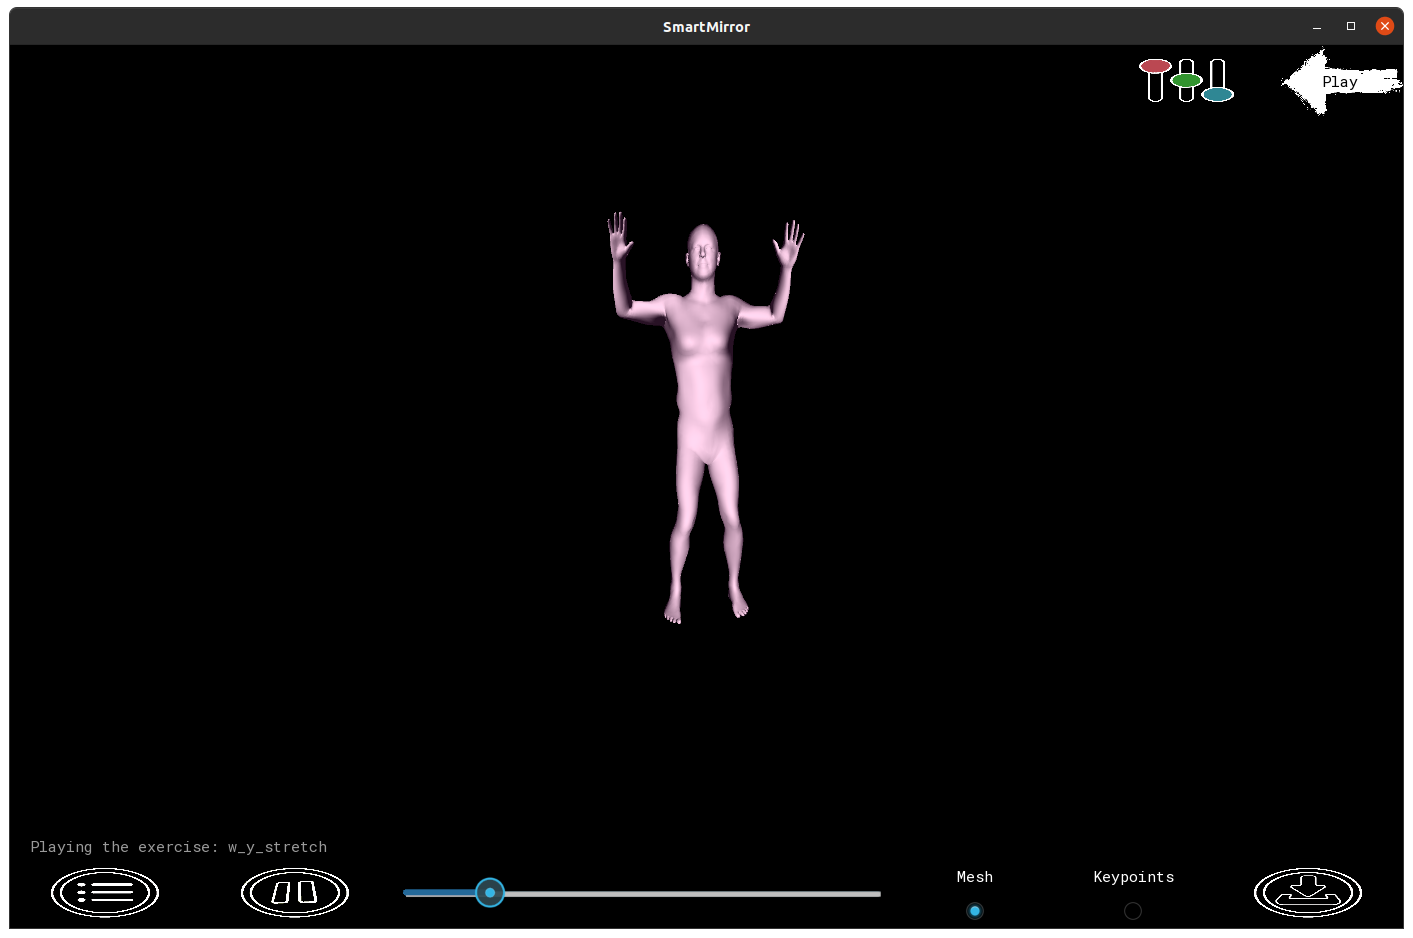
\includegraphics[width=\textwidth]{images/chapter5/render_mesh.png}
		\caption{Απεικόνιση του πλέγματος.}
	\end{subfigure}
	\hfill
	\begin{subfigure}[h]{0.45\textwidth}
		\centering
		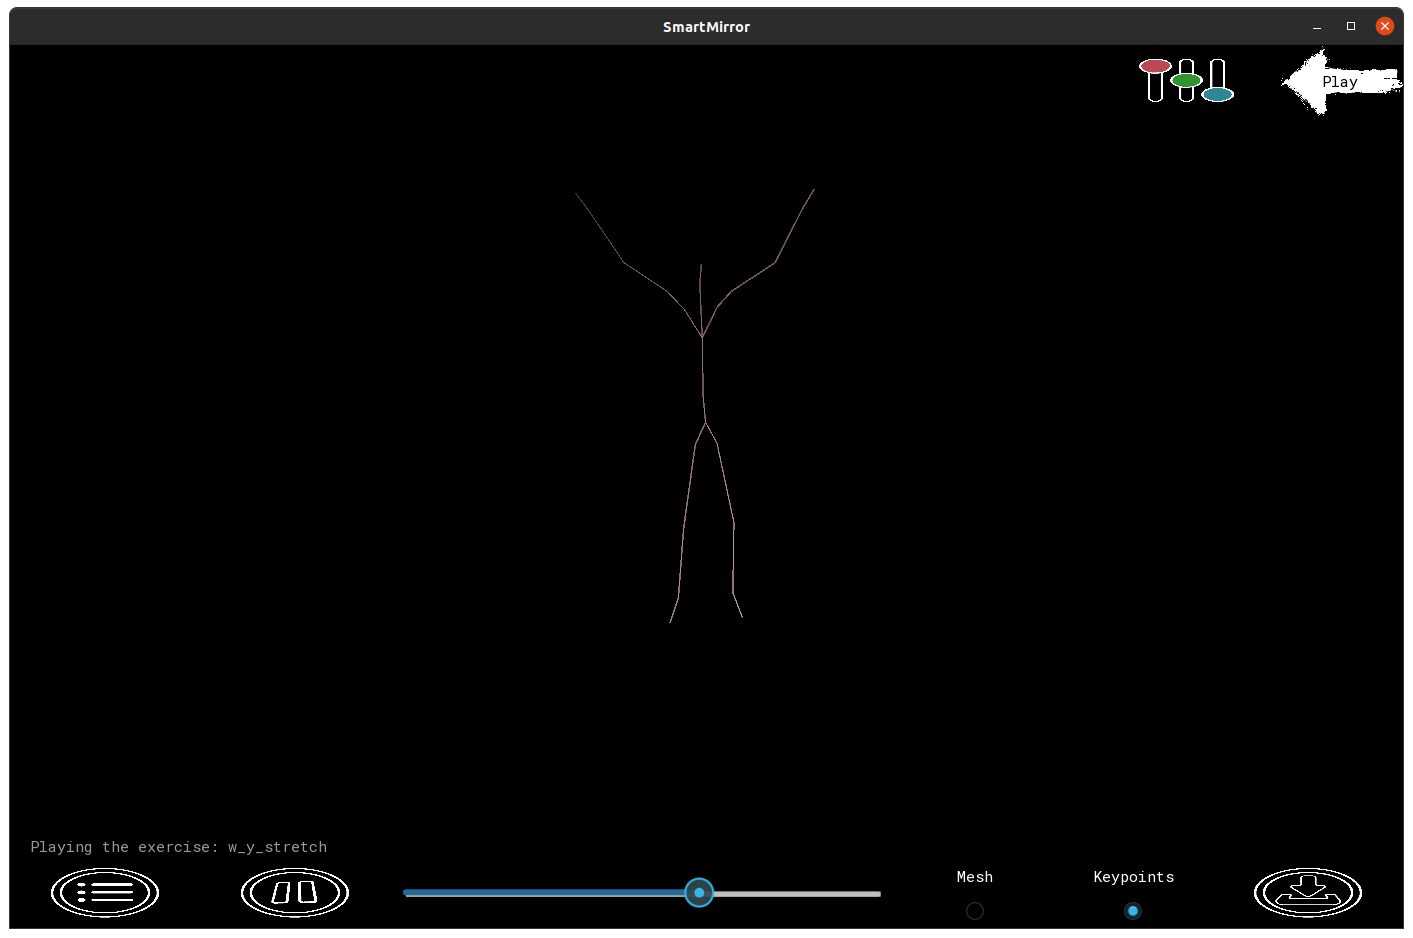
\includegraphics[width=\textwidth]{images/chapter5/render_kpnt.png}
		\caption{Απεικόνιση του σκελετού}
	\end{subfigure}
	\caption{Οι τρόποι απεικόνισης του ανθρώπου.}
	\label{fig:render_options}
\end{figure}

\noindent\textbf{Μέθοδοι Κλάσης}
\begin{itemize}
	\item \texttt{\_\_init\_\_(actions, info\_label)}: Αποθηκεύει τα χαρακτηριστικά \texttt{actions} και \texttt{info\_label} και θέτει την προεπιλεγμένη τιμή του \texttt{smpl\_mode} σε 'smpl\_mesh'.
	\item \texttt{on\_play\_pause(state)}: Όταν το \texttt{state} είναι 'normal' κάνει παύση όλα τα \texttt{actions}. Όταν είναι 'down' συνεχίζει τα \texttt{actions} που ήταν ενεργοποιημένα. Αν δεν υπήρχε κανένα ενεργοποιημένο \texttt{action} τότε η κατάσταση του κουμπιού δεν αλλάζει.
	\item \texttt{reset\_ui()}: Επαναφέρει την γραφική διεπαφή των κουμπιών στην αρχική τους κατάσταση και κλείνει ενδεχομένως ανοιχτούς διαλόγους.
	\item \texttt{set\_smpl\_mode(mode, is\_active)}: Όταν το \texttt{is\_active} είναι αληθές, αλλάζει τον τρόπο απεικόνισης του ανθρώπου σε πλέγμα ή σκελετό ανάλογα με την τιμή του \texttt{mode}.
	\item \texttt{start\_exercise(exercise\_name)}: Αρχίζει την αναπαραγωγή της άσκησης με όνομα \texttt{exercise\_name}, θέτοντας την τιμή του \texttt{current\_exercise} του αντικειμένου \texttt{ExerciseController}. Σταματάει το \texttt{PredictAction} και ξεκινάει το \texttt{PlayAction} ή το \texttt{PlaybackAction} αν είμαστε στην κλάση \texttt{PlayControls} ή \texttt{EditorControls} αντίστοιχα.
	\item \texttt{update(exercise\_controller)}: Αναβαθμίζει τα δεδομένα των διαθέσιμων ασκήσεων. Καλείται από το αντικείμενο \texttt{Exercise Controller} όταν αλλάζουν τα δεδομένα.
\end{itemize}

\subsubsection{PlayControls}
Τα κουμπιά της κλάσης \texttt{PlayControls} από τα αριστερά προς τα δεξιά, όπως φαίνονται στο Σχήμα \ref{fig:play_controls} είναι
\begin{itemize}
	\item Κουμπί επιλογής ασκήσεως αναφοράς για την έναρξη \textsl{παιχνιδιού}.
	\item Κουμπί παύσης ή συνέχισης της αναπαραγόμενης άσκησης.
	\item Διακόπτης επιλογής του τρόπου απεικόνισης του ανθρώπινου μοντέλου άσκησης αναφοράς.
\end{itemize}

\noindent\textbf{Μέθοδοι Κλάσης}
\begin{itemize}
	\item \texttt{demo\_render(rendered\_obj)}: Μέθοδος για αποσφαλμάτωση του απεικονιστή κλάσης \texttt{Renderer} \ref{sec:renderer}. Η τιμή του \texttt{rendered\_obj} μπορεί να είναι 'smpl' ή 'monkey' όπου στην πρώτη περίπτωση γίνεται απεικόνιση του ανθρώπου από την εκτίμηση πόζας χωρίς καμία επιπλέον λειτουργία, ενώ στην δεύτερη περίπτωση γίνεται απεικόνιση ενός πλέγματος διαβασμένο από αρχείο κατάληξης \texttt{.obj}.
\end{itemize}

\subsubsection{EditorControls}
\noindent\textbf{Περιγραφή Κλάσης}
Η κλάση \texttt{EditorControls} έχει όλα τα κουμπιά που έχει και η \texttt{PlayControls}, όπως φαίνεται στο Σχήμα \ref{fig:editor_controls} αλλα επιπλέον περιλαμβάνει:
\begin{itemize}
	\item Έναν ολισθητή ο οποίος δείχνει το τωρινό καρέ της άσκησης και μέσω αυτού μπορεί να ελεγχθεί η αναπαραγωγή της άσκησης.
	\item Ένα κουμπί με το οποίο ανοίγει ένας διάλογος επιλογής αρχείου βίντεου, μέσω του οποίου γίνεται η εκτίμηση πόζας και η αποθήκευση των δεδομένων ως ασκήσεως αναφοράς.
	\item Με μονό κλικ κατά την αναπαραγωγή ασκήσεως αναφοράς ανοίγει ένας διάλογος δίνοντας την δυνατότητα επεξεργασίας της περιστροφής οποιασδήποτε άρθρωσης - σημείου κλειδιού, όπως φαίνεται στο Σχήμα \ref{fig:edit_keypoint}
\end{itemize}

\noindent\textbf{Χαρακτηριστικά κλάσης}
\begin{itemize}
	\item \texttt{frame\_indx}: Ο δείκτης του τωρινού καρέ. Ελέγχει την τιμή στην οποία βρίσκεται ο ολισθητής, που είναι κλάσης \texttt{kivy.uix.slider.Slider}\footnote{\href{https://kivy.org/doc/stable/api-kivy.uix.slider.html}{https://kivy.org/doc/stable/api-kivy.uix.slider.html}}.
	\item \texttt{user\_touching\_slider}: Εάν ο χρήστης ακουμπάει αυτή την στιγμή τον ολισθητή.
	\item \texttt{was\_playing}: Εάν η αναπαραγωγή της άσκησης ήταν σε κατάσταση παύσης ή όχι όταν ξεκίνησε το κλικ, \texttt{on\_touch\_down()}.
\end{itemize}

\noindent\textbf{Μέθοδοι Κλάσης}
\begin{itemize}
	\item \texttt{dismiss\_keypoint\_edit\_form()}: Κλείνει τον διάλογο κλάσης \texttt{KeypointEditForm}.
	\item \texttt{dismiss\_load\_dialog()}: Κλείνει τον διάλογο επιλογής βίντεο.
	\item \texttt{display\_kpnt\_edit\_form(kpnt\_name, keypoints\_spec)}: Ανοίγει τον διάλογο \texttt{KeypointEditForm} στο σημείο κλειδί \texttt{kpnt\_name}. Επίσης, δίνει στον διάλογο όλες τις πληροφορίες για τα διαθέσιμα σημεία κλειδιά \texttt{keypoints\_spec}.
	\item \texttt{on\_frame\_indx(instance, value)}: Καλείται όταν αλλάζει το \texttt{frame\_indx} θέτοντας το \texttt{frame\_indx} του διαλόγου \texttt{KeypointEditForm} αν υπάρχει.
	\item \texttt{on\_slider\_value(instance, value)}: Καλείται όταν αλλάζει το \texttt{frame\_indx} λόγω του κλικ του χρήστη. Θέτει το τωρινό καρέ της αναπαραγόμενης άσκησης στην τιμή \texttt{value}.
	\item \texttt{on\_touch\_down(touch)}: Όταν ο χρήστης κάνει κλικ αν είναι μέσα στον χώρο του ολισθητή θέτει την true στο \texttt{user\_touching\_slider} και κρατάει την κατάσταση παύσης ή όχι του action στο \texttt{was\_playing}.
	\item \texttt{on\_touch\_up(touch)}: Συνεχίζει την αναπαραγωγή από την κατάσταση που ήταν πριν το \texttt{on\_touch\_down()}.
	\item \texttt{predit\_from\_video(path, filename)}: Εκτελείται όταν ο χρήστης διαλέξει ένα βίντεο από τον διάλογο \texttt{LoadDialog}. Αρχικά καλεί την \texttt{dismiss\_load\_dialog()} και στην συνέχεια ξεκινάει το action \texttt{PredictAction}, σταματώντας ενδεχομένως το \texttt{PlaybackAction}, με είσοδο το αρχείο, αν υπάρχει, στο \texttt{path/filename}. Έπειτα, γίνεται η εκτίμηση πόζας και τα δεδομένα του βίντεο αποθηκεύονται ως δεδομένα άσκησης αναφοράς.
	\item \texttt{save\_kpnt\_rules()}: Αποθηκεύει τους κανόνες που τέθηκαν από το \texttt{KeypointEditForm} και κλείνει τον διάλογο καλώντας την \texttt{dismiss\_kpnt\_edit\_form()}. Σημειώνεται ότι η αποθήκευση στον δίσκο των κανόνων δεν έχει υλοποιηθεί, αλλά αποθηκεύονται μόνο στην μνήμη.
	\item \texttt{show\_load\_dialog()}: Ανοίγει τον δίαλογο \texttt{LoadDialog}. 
\end{itemize}

\begin{figure}[h]
	\centering
	\begin{subfigure}[h]{0.45\textwidth}
	\centering
		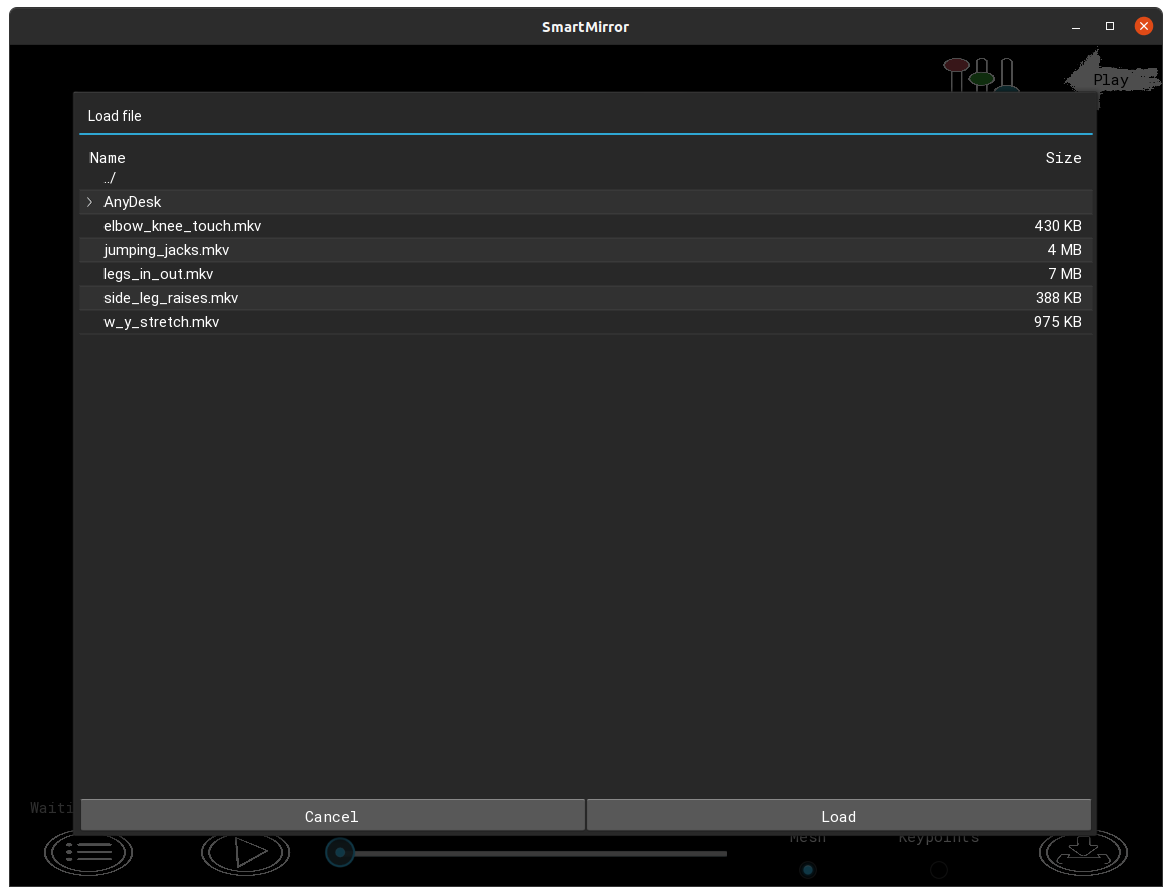
\includegraphics[width=\textwidth]{images/chapter5/load_dialog.png}
		\caption{Γραφική αναπαράσταση του \texttt{LoadDialog}, o διάλογος επιλογής βίντεο προς εισαγωγή ως ασκήσεως αναφοράς.}
		\label{fig:load_dialog_ui}
	\end{subfigure}
	\hfill
	\begin{subfigure}[h]{0.45\textwidth}
	\centering
		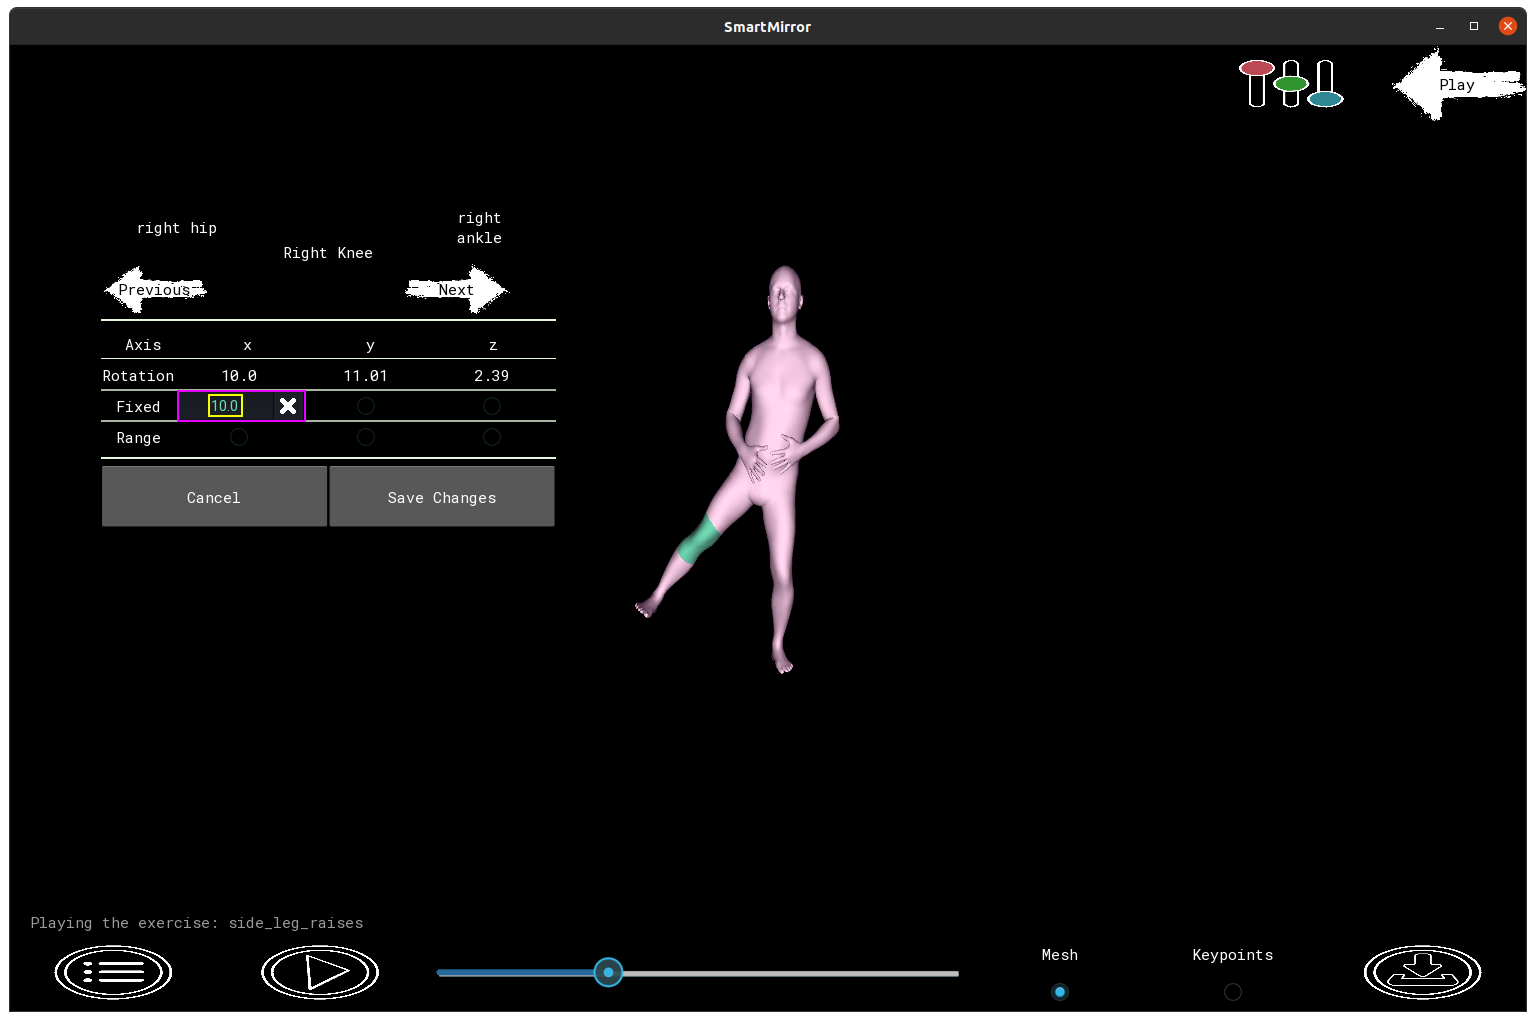
\includegraphics[width=\textwidth]{images/chapter5/editing_form.png}
		\caption{Γραφική αναπαράσταση του \texttt{EditKeypointForm}, o διάλογος επεξεργασίας περιστροφής σημείου κλειδιού. Στο ροζ ορθογώνιο φαίνεται η κλάση \texttt{RotInputForm} ενώ στο κίτρινο η \texttt{RotInputText}.}
		\label{fig:edit_keypoint}
	\end{subfigure}
	\caption{Οι διαθέσιμοι διάλογοι της κλάσης \texttt{EditorControls}.}
	\label{fig:editor_dialogs}
\end{figure}

\subsubsection{KeypointEditForm}
Για χάρη συντομίας δεν θα αναλύσουμε διεξοδικά τις μεθόδους και μεταβλητές της κλάσης καθώς είναι κυρίως γραφικές κλάσεις με λειτουργικότητα που αφορά μόνο την εμφάνιση και έλεγχο των checkboxes και των φορμών εισόδου γωνιών περιστροφής για την διαχείριση των κανόνων.

\noindent\textbf{Περιγραφή Κλάσης}

Η κλάση \texttt{KeypointEditForm} μαζί με τις \texttt{RotInputForm} και \texttt{RotTextInput} φαίνονται στο Σχήμα \ref{fig:edit_keypoint}. Ανάλογα με το διαλεγμένο σημείο κλειδί καλείται η μέθοδος \texttt{\_setup\_highlight()} για την εμφάνιση της τιρκουάζ περιοχής πάνω στο ανθρώπινο πλέγμα. Η επιλογή του σημείου κλειδιού γίνεται με κλικ στο πλέγμα, όπου επιλέγεται το κοντινότερο σημείο, ή με τα βελάκια \textsl{Previous} και \textsl{Next} που καλούνε τις μεθόδους \texttt{cycle\_prev()} και \texttt{cycle\_next()} για να πάνε στο προηγούμενο ή επόμενο σημείο κλειδί αντίστοιχα.

Στην φόρμα, φαίνονται οι περιστροφές σε μοίρες ανά καρέ, γύρω κάθε άξονα για το επιλεγμένο σημείο κλειδί. Για την εισαγωγή ενός κανόνα, αρκεί ο χρήστης να κάνει κλικ στο checkbox στην στήλη του άξονα και στην γραμμή ανάλογα με τον κανόνα που επιθυμεί. Τότε, το checkbox μετατρέπεται σε ένα πεδίο εισόδου κειμένου, όπου μπορεί να πληκτρολογήσει γωνίες και να θέσει τον κανόνα, είτε να πατήσει το \texttt{Χ} και να σβήσει τον κανόνα.

Στην περίπτωση εισόδου κανόνα \textsl{fixed} ο χρήστης μπορεί να πληκτρολογήσει μόνο έναν αριθμό, που είναι η σταθερή γωνία περιστροφής γύρω από τον άξονα για αυτό το σημείο κλειδί. Αντίθετα, στην περίπτωση κανόνα \textsl{range}, ο χρήστης μπορεί να βάλει 2 γωνίες με την μορφή \textit{angle1:angle2}, όπου καθορίζεται το διάστημα μοιρών μέσα στο οποίο μπορεί να κινηθεί το σημείο κλειδί.

\subsection{Actions}
\label{sec:abstract_actions}

\begin{figure}[h]
	\centering
	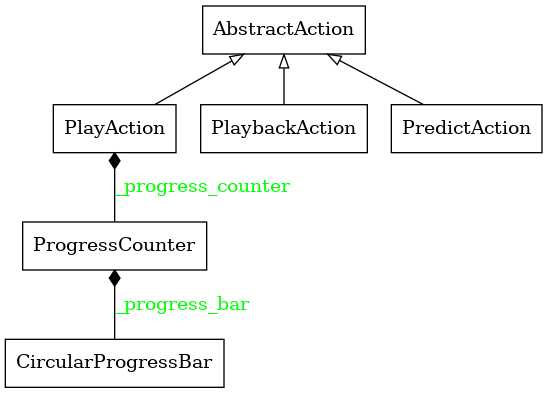
\includegraphics[scale=0.7]{images/chapter5/actions_overview.png}
	\caption{Εποπτικό UML διάγραμμα των κλάσεων τύπου \texttt{AbstractActions} και των σχέσεων τους.}
	\label{fig:actions_overview}
\end{figure}

Οι κλάσεις τύπου \texttt{AbstractAction} είναι οι ελεγκτές των διαφορετικών λειτουργιών που απαιτούν μοντέλα μηχανικής μάθησης. Το κάθε action είναι υπεύθυνο για την διαχείριση των μοντέλων που είναι αναγκαία για την διεκπεραίωση της λειτουργίας του. Δέχεται τα δεδομένα των εκτιμήσεων και περνάνε τα δεδομένα στις κλάσεις \texttt{Renderer}, \ref{sec:renderer} για την απεικόνιση τους.

Αναλυτικότερα, οι διαθέσιμες ενέργειες, actions, είναι η απλή εκτίμηση πόζας, \texttt{PredictAction}, η αναπαραγωγή αποθηκευμένης άσκησης αναφοράς, \texttt{PlaybackAction}, και η λειτουργία \textsl{παιχνιδιού}, \texttt{PlayAction}.


\subsubsection{AbstractAction}

\begin{figure}[H]
	\centering
	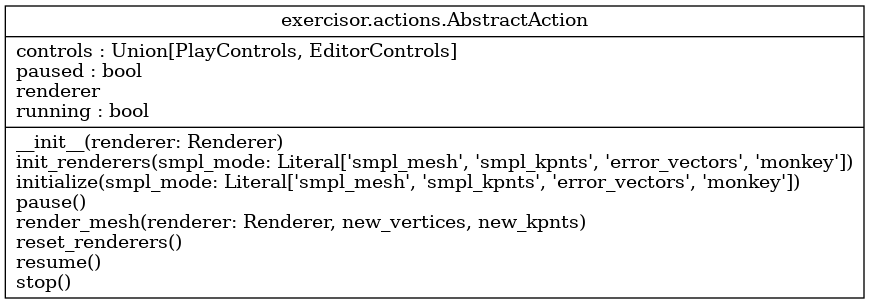
\includegraphics[scale=0.5]{images/chapter5/abstract_action_uml.png}
	\caption{UML διάγραμμα της κλάσης \texttt{AbstractAction}.}
	\label{fig:abstract_action}
\end{figure}

\noindent\textbf{Περιγραφή Κλάσης}
Το κάθε action χαρακτηρίζεται από 2 καταστάσεις, τις \textsl{running} και \textsl{paused}. Η κατάσταση \textsl{running} δηλώνει αν το συγκεκριμένο action είναι το ενεργό, ενώ η κατάσταση \textsl{paused} αν το action είναι σε παύση, δηλαδή δεν γίνεται κάποια εκτίμηση αυτή την στιγμή.

\noindent\textbf{Χαρακτηριστικά κλάσης}
\begin{itemize}
	\item \texttt{controls}: Αναφορά σε αντικείμενο τύπου \texttt{PlayControls} ή \texttt{EditorControls}.
	\item \texttt{renderer}: Αντικείμενο κλάσης \texttt{Renderer} το οποίο λειτουργεί ως ο κύριος απεικονιστής των εκτιμήσεων που παράγονται από τα μοντέλα μηχανικής μάθησης.
	\item \texttt{paused}: Μεταβλητή που δηλώνει αν το action βρίσκεται στην κατάσταση \textsl{paused} ή όχι.
	\item \texttt{running}: Μεταβλητή που δηλώνει αν το action βρίσκεται στην κατάσταση \textsl{running} ή όχι.
\end{itemize}

\noindent\textbf{Μέθοδοι Κλάσης}
\begin{itemize}
	\item \texttt{init\_renderers(smpl\_mode)}: Αρχικοποιεί τον \texttt{renderer} ορίζοντας το αντικείμενο που θα απεικονιστεί.
	\item \texttt{initialize(smpl\_mode)}: Ενεργοποιεί την ενέργεια. Αρχικά, καλεί την μέθοδο \texttt{stop()}, καλεί την \texttt{init\_renderers()} και Θέτει την \texttt{running} σε true και τρέχει την \texttt{resume()}.
	\item \texttt{pause()}: Θέτει την \texttt{paused} σε true και αν υπάρχει η \texttt{controls} βάζει το \textit{Play\\Pause} κουμπί στην κατάσταση παύσης.
	\item \texttt{render\_mesh(renderer, new\_vertices, new\_kpnts)}: Θέτει τις κορυφές του απεικονιστή \texttt{renderer} στις τιμές είτε των \texttt{new\_vertices} είτε των \texttt{new\_kpnts}, ανάλογα με το ποιο υπάρχει.
	\item \texttt{reset\_renderers()}: Καλεί την συνάρτηση \texttt{reset\_scene()} \textbf{όλων} των αντικειμένων \texttt{Renderer} που υπάρχουν στην οθόνη.
	\item \texttt{resume()}: Θέτει την \texttt{paused} σε false και αν υπάρχει η \texttt{controls} βάζει το \textit{Play\\Pause} κουμπί στην κατάσταση συνέχειας. 
	\item \texttt{stop()}: Θέτει την \texttt{running} σε false καλεί την \texttt{reset\_renderers()} και αν υπάρχει η \texttt{controls} καλεί την μέθοδο της \texttt{reset\_ui()}.
\end{itemize}

\subsubsection{PredictAction}

\begin{figure}[H]
	\centering
	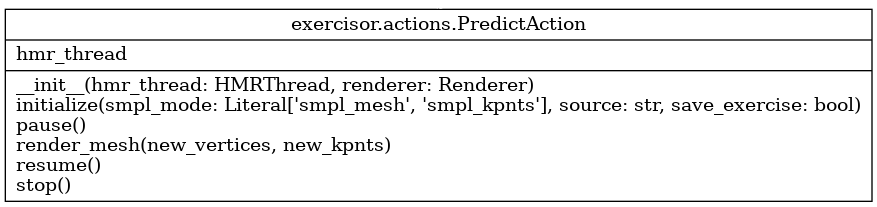
\includegraphics[scale=0.5]{images/chapter5/predict_action_uml.png}
	\caption{UML διάγραμμα της κλάσης \texttt{PredictAction}.}
	\label{fig:predict_action}
\end{figure}

\noindent\textbf{Περιγραφή Κλάσης}
Η κλάση \texttt{PredictAction} διαχειρίζεται ένα αντικείμενο κλάσης \texttt{HMRThread} για την διεκπεραίωση της απλής εκτίμησης πόζας και απεικόνισης των αποτελεσμάτων. Η ενέργεια αυτή χρησιμοποιείται για την εκτίμηση των δεδομένων ασκήσεως αναφοράς από ένα βίντεο.

\noindent\textbf{Χαρακτηριστικά κλάσης}
\begin{itemize}
	\item \texttt{hmr\_thread}: Αναφορά σε αντικείμενο κλάσης \texttt{HMRThread}, \ref{sec:hmr_thread}.
\end{itemize}

\noindent\textbf{Μέθοδοι Κλάσης}

Οι μέθοδοι \texttt{pause()} και \texttt{stop()} σταματάνε την λειτουργία του \texttt{HMRThread} ενώ η \texttt{resume()} την συνεχίζει.
\begin{itemize}
	\item \texttt{initialize(smpl\_mode, source, save\_exercise)}: Καλεί την μέθοδο \texttt{initialize()} της \texttt{AbstractAction} και θέτει την συνάρτηση εξόδου του \texttt{HMRThread} να είναι η μέθοδος \texttt{render\_mesh()}. Επίσης, θέτει την πηγή εισόδου βίντεο του \texttt{HMRThread} που μπορεί να είναι είτε \textsl{"cam"}\footnote{Η λειτουργία αυτή χρησιμοποιήθηκε για αποσφαλμάτωση.}, όπου γίνεται εκτίμηση από την κάμερα του χρήστη, είτε το path από ένα αρχείο βίντεο. Αν η \texttt{save\_exercise} είναι true, τότε όταν τελειώσει η αναπαραγωγή αποθηκεύονται όλα τα εκτιμώμενα δεδομένα.
	\item \texttt{render\_mesh(new\_vertices, new\_kpnts)}: Καλεί την συνάρτηση \texttt{render\_mesh} της \texttt{AbstractAction} με όρισμα \texttt{renderer} το χαρακτηριστικό \texttt{renderer} του αντικειμένου.
\end{itemize}


\subsubsection{PlaybackAction}

\begin{figure}[H]
	\centering
	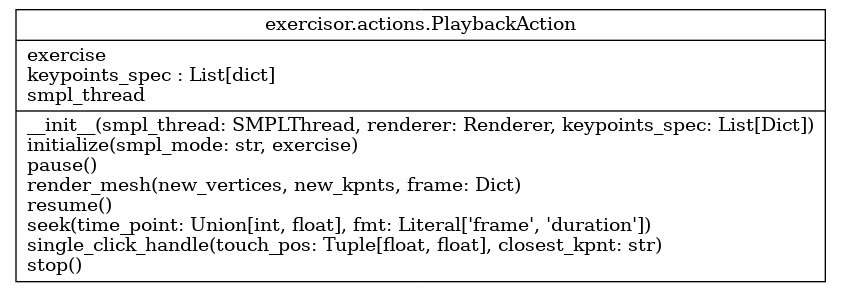
\includegraphics[scale=0.5]{images/chapter5/playback_action_uml.png}
	\caption{UML διάγραμμα της κλάσης \texttt{PlaybackAction}.}
	\label{fig:playback_action}
\end{figure}

\noindent\textbf{Περιγραφή Κλάσης}
Η κλάση \texttt{PlaybackAction} διαχειρίζεται ένα αντικείμενο κλάσης \texttt{SMPLThread} για την μετατροπή των παραμέτρων SMPL σε κορυφές πλέγματος ανθρώπου και σκελετού προς απεικόνιση. Η ενέργεια αυτή χρησιμοποιείται για την αναπαραγωγή μιας αποθηκευμένης άσκησης αναφοράς στην λειτουργία \textsl{επιμελητή}.

\noindent\textbf{Χαρακτηριστικά κλάσης}
\begin{itemize}
	\item \texttt{exercise}: O πίνακας $Ν \times 82$ με τις 82 παραμέτρους SMPL για κάθε καρέ από τα N.
	\item \texttt{keypoints\_spec}: Τα χαρακτηριστικά των διαθέσιμων σημείων κλειδιών από το μοντέλο SMPL.
	\item \texttt{smpl\_thread}: Αναφορά σε αντικείμενο κλάσης \texttt{SMPLThread}, \ref{sec:smpl_thread}.
\end{itemize}

\noindent\textbf{Μέθοδοι Κλάσης}

Οι μέθοδοι \texttt{pause()} και \texttt{stop()} σταματάνε την λειτουργία του \texttt{SMPLThread} ενώ η \texttt{resume()} την συνεχίζει.
\begin{itemize}
	\item \texttt{\_\_init\_\_(smpl\_thread, renderer, keypoints\_spec): Θέτει στον \texttt{renderer} να εκτελεί την μέθοδο \texttt{single\_click\_handle}} όταν γίνεται ένα κλικ.
	\item \texttt{initialize(smpl\_mode, exercise)}: Καλεί την \texttt{initialize} της \texttt{AbstractControl}, θέτει την μέθοδο εξόδου του \texttt{SMPLThread} να είναι η \texttt{render\_mesh()}, θέτοντας επίσης τα δεδομένα της άσκησης που θα γίνει αναπαραγωγή.
	\item \texttt{render\_mesh(new\_vertices, new\_kpnts, frame)}: Καλεί την συνάρτηση \texttt{render\_mesh} της \texttt{AbstractAction} με όρισμα \texttt{renderer} το χαρακτηριστικό του αντικειμένου. Επίσης, θέτει το \texttt{frame\_indx} του \texttt{EditorControls} σύμφωνα με το \texttt{frame}\footnote{Το \texttt{frame} περιλαμβάνει πληροφορίες για το καρέ όπως τον δείκτη και την χρονική στιγμή που λήφθηκε.} ώστε να αντικατοπτρίζει το καρέ που μόλις απεικονίστηκε.
	\item \texttt{seek(time\_point, fmt)}: Μέθοδος μέσω της οποίας ελέγχεται το σημείο καρέ της αναπαραγωγής. Αν το \texttt{fmt} είναι \textsl{"frame"} τότε θέτει το \texttt{frame\_indx} του \texttt{SMPLThread} και του \texttt{EditorControls} σε αυτόν τον αριθμό. Αν το \texttt{fmt} είναι \textsl{"duration"} τότε η αναπαραγωγή πηγαίνει πίσω ή μπροστά τόσα δευτερόλεπτα (ανάλογα με το πρόσημο του \texttt{time\_point}).
	\item \texttt{single\_click\_handle(touch\_pos, closest\_kpnt)}: Εκτελεί την μέθοδο \texttt{display\_kpnt\_edit\_form} του \texttt{EditorControls} με όρισμα το όνομα του πιο κοντινού σημείου κλειδιού \texttt{closest\_kpnt}.
\end{itemize}


\subsubsection{PlayAction}

\begin{figure}[H]
	\centering
	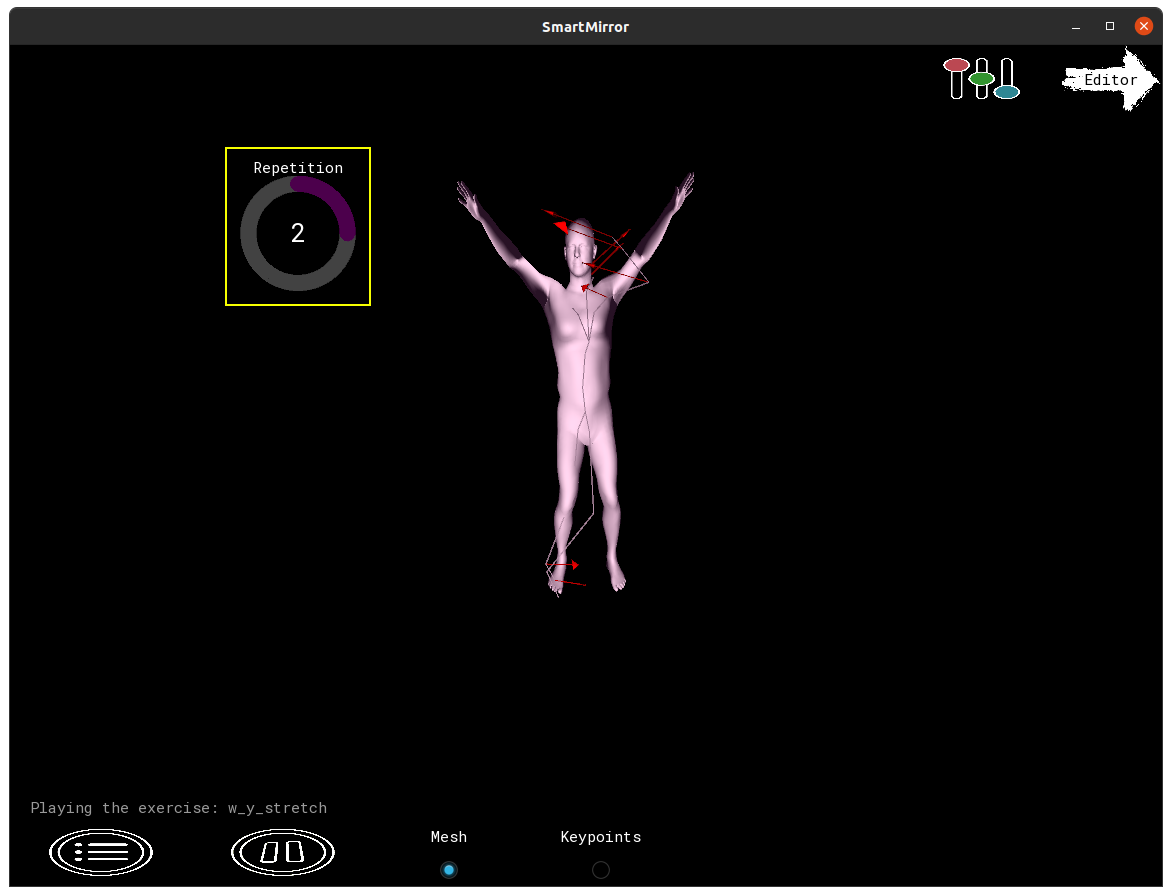
\includegraphics[scale=0.38]{images/chapter5/playing_action.png}
	\caption{Γραφική απεικόνιση της λειτουργίας \textsl{παιχνιδιού}. Το ανθρώπινο πλέγμα είναι η απεικόνιση της άσκηση αναφοράς ενώ με τον σκελετό απεικονίζεται η εκτίμηση πόζας του χρήστη. Στο κίτρινο ορθογώνιο φαίνεται το widget \texttt{ProgressCounter}.}
	\label{fig:play_action}
\end{figure}

\begin{figure}[H]
	\centering
	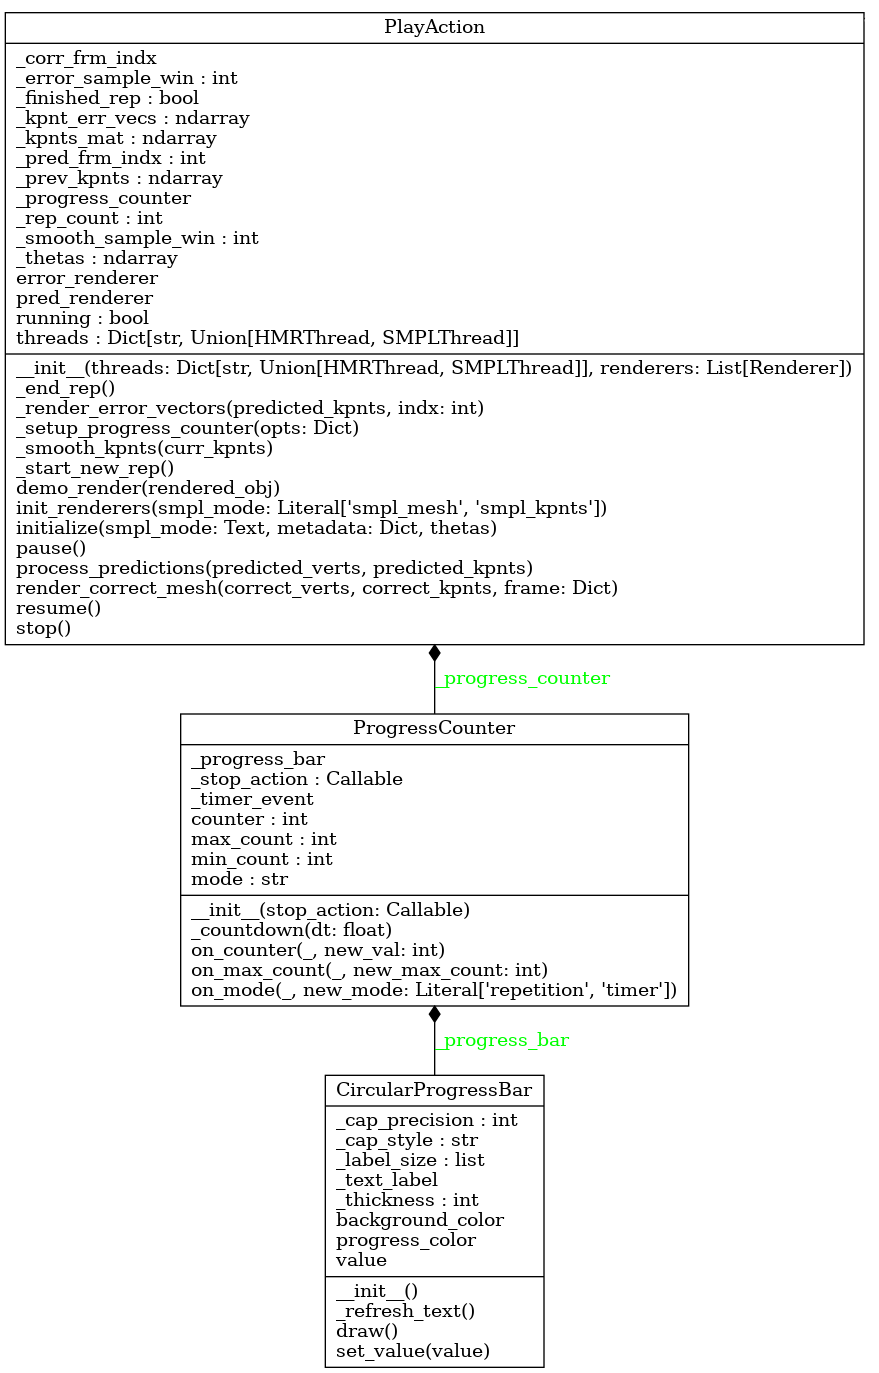
\includegraphics[scale=0.4]{images/chapter5/play_action_uml.png}
	\caption{UML διάγραμμα της κλάσης \texttt{PlayAction}.}
	\label{fig:play_action}
\end{figure}

\noindent\textbf{Περιγραφή Κλάσης}

Η ενέργεια \texttt{PlayAction} ελέγχει την κυρίως λειτουργία \textsl{παιχνιδιού} της εφαρμογής. Χρησιμοποιεί ταυτόχρονα τα threads \texttt{HMRThread} και \texttt{SMPLThread} για την εκτίμηση πόζας του χρήστη από την κάμερα και την αναπαραγωγή της άσκησης αναφοράς αντίστοιχα. Το κάθε thread απεικονίζει τα αποτελέσματα στον δικό του \texttt{renderer}. Ένας τρίτος \texttt{renderer} χρησιμοποιείται για την απεικόνιση διορθωτικών βελών ή διανυσμάτων σφάλματος, δείχνοντας από την πόζα του χρήστη στην πόζα αναφοράς για κάθε σημείο κλειδί. Τα διορθωτικά βέλη και οι εκτιμήσεις του μοντέλου \texttt{HMR} χρησιμοποιούν έναν αλγόριθμο κινούμενου μέσου όρου στα τελευταία καρέ για να αντισταθμίσουν ενδεχόμενες ακραίες εκτιμήσεις και να εξομαλύνουν την απεικόνιση. Η λειτουργία \textsl{παιχνιδιού} φαίνεται στο Σχήμα \ref{fig:play_action}.

Τέλος, ένα επιπλέον widget, κλάσης \texttt{ProgressCounter}, λειτουργεί ως μετρητής του αριθμού των επαναλήψεων ή ως αντίστροφος χρονομετρητής που καθορίζεται από το χαρακτηριστικό του \texttt{mode}. Τα \texttt{max\_count} και \texttt{min\_count} είναι τα όρια του μετρητή. Όταν φτάσει σε κάποιο από τα όρια ανάλογα με την λειτουργία του εκτελείται η \texttt{\_stop\_action} που του έχει δοθεί στην αρχικοποίηση για να σταματήσει η ενέργεια. Η κλάση \texttt{CircularProgressBar} υλοποιεί την γραφική διεπαφή του μετρητή. 


\noindent\textbf{Χαρακτηριστικά κλάσης}
\begin{itemize}
	\item \texttt{threads}: Αναφορές σε αντικείμενα κλάσης \texttt{HMRThread} και \texttt{SMPLThread}.
	\item \texttt{\_corr\_frm\_indx}: Ο δείκτης καρέ που βρίσκεται το \texttt{SMPLThread}.
	\item \texttt{\_error\_sample\_win}: Το παράθυρο του κινούμενου μέσου όρου σε αριθμό καρέ για την ομαλοποίηση των διανυσμάτων σφάλματος (error vectors).
	\item \texttt{\_finished\_rep}: Μεταβλητή boolean που δηλώνει πότε η αναπαραγωγή από το \texttt{SMPLThread} φτάνει στο τέλος της.
	\item \texttt{\_kpnt\_err\_vecs}: Πίνακας διαστάσεων $N \times 24 \times 3$ όπου αποθηκεύονται οι 3 συντεταγμένες των διανυσμάτων σφάλματος των 24 σημείων κλειδιών για τα N καρέ της άσκησης.
	\item \texttt{\_kpnts\_mat}: Πίνακας $Ν \times 24 \times 3$ που αποθηκεύονται από το \texttt{SMPLThread} οι σωστές 3 συντεταγμένες των 24 σημείων κλειδιών για τα Ν καρέ.
	\item \texttt{\_pred\_frm\_indx}: Ο αριθμός των εκτιμήσεων του \texttt{HMRThread} που έχουν γίνει.
	\item \texttt{\_prev\_kpnts}: Πίνακας διαστάσεων (\_smooth\_sample\_window$\times 24 \times 3$) που αποθηκεύονται οι 3 συντεταγμένες των 24 σημείων κλειδιών για την εφαρμογή του κινούμενου μέσου όρου.
	\item \texttt{\_progress\_counter}: Αντικείμενο της κλάσης \texttt{ProgressCounter}.
	\item \texttt{\_rep\_count}: Μετρητής του αριθμού επαναλήψεων.
	\item \texttt{\_smooth\_sample\_win}: Το παράθυρο του κινούμενου μέσου όρου σε αριθμό καρέ για την ομαλοποίηση των εκτιμήσεων του \texttt{HMRThread}.
	\item \texttt{\_thetas}: Τα δεδομένα της άσκησης αναφοράς, πίνακας $Ν \times 82$ των 82 παραμέτρων SMPL για τα Ν καρέ.
\end{itemize}

\noindent\textbf{Μέθοδοι Κλάσης}
\begin{itemize}
	\item \texttt{\_end\_rep()}: Υπολογίζει το συνολικό μέσο τετραγωνικό σφάλμα της επανάληψης και εκτελεί την μέθοδο \texttt{play\_animation} του \texttt{renderer}.
	\item \texttt{\_render\_error\_vectors(predicted\_kpnts, indx)}: Υπολογίζει τον κινούμενο μέσο όρο των διανυσμάτων σφάλματος στον δείκτη καρέ \texttt{indx} και απεικονίζει τα διανύσματα που έχουν μέτρο μεγαλύτερο από μία τιμή.
	\item \texttt{\_setup\_progress\_counter(opts)}: Αρχικοποιεί τον μετρητή \texttt{ProgressCounter} στην λειτουργία μετρητή ή αντίστροφου χρονομέτρου.
	\item \texttt{\_smooth\_kpnts(curr\_kpnts)}: Εφαρμόζει τον κινούμενο μέσο όρο στις εκτιμήσεις \texttt{curr\_kpnts}.
	\item \texttt{\_start\_new\_rep()}: Επαναφέρει στις αρχικές τιμές τα χαρακτηριστικά \texttt{\_pred\_frm\_indx}, \texttt{\_finished\_rep}, \texttt{\_kpnts\_mat}, \texttt{\_kpnt\_err\_vecs}, αυξάνει το \texttt{\_rep\_count} κατά ένα και καλεί την \texttt{reset\_scene} του \texttt{error\_renderer}.
	\item \texttt{init\_renderers(smpl\_mode)}: Θέτει τον \texttt{smpl\_renderer} στον τρόπο απεικόνισης που ορίζεται από το \texttt{smpl\_mode} και τον \texttt{pred\_renderer} στον αντίθετο. 
	\item \texttt{initialize(smpl\_mode, metadata, thetas)}: Θέτει τις μεθόδους εξόδου των \texttt{SMPLThread} και \texttt{HMRThread} στις μεθόδους \texttt{render\_correct\_mesh()} \texttt{process\_predictions()} αντίστοιχα. Θέτει την άσκηση αναφοράς \texttt{\_thetas} στο \texttt{SMPLThread} το \texttt{\_rep\_count} στο 0, αρχικοποιεί τον \texttt{ProgressCounter} καλώντας την \texttt{\_setup\_progress\_counter()} και καλεί την \texttt{\_start\_new\_rep()}.
	\item \texttt{process\_predictions(predicted\_verts, predicted\_kpnts)}: Καλεί την \texttt{\_smooth\_kpnts} στις εκτιμήσεις, υπολογίζει τα διανύσματα σφάλματος και τα αποθηκεύει, αυξάνει την \texttt{\_pred\_frm\_indx}, απεικονίζει τα αποτελέσματα καλώντας την \texttt{render\_mesh()} του \texttt{AbstractAction} και ελέγχει την \texttt{\_finished\_rep}, όπου αν τελείωσε η επανάληψη για να εκτελέσει τις \texttt{\_end\_rep()} και \texttt{\_start\_new\_rep()}.
	\item \texttt{render\_correct\_mesh(correct\_verts, correct\_kpnts, frame)}: Αποθηκεύει τις σωστές εκτιμήσεις για το συγκεκριμένο καρέ, απεικονίζει τα αποτελέσματα καλώντας την \texttt{render\_mesh()} του \texttt{AbstractAction} και ελέγχει αν το καρέ είναι το τελευταίο οπότε θέτει την \texttt{\_finished\_rep} σε true.
\end{itemize}

\newpage
\subsection{MLThreads}
\label{sec:ml_threads}

\begin{figure}[H]
	\centering
	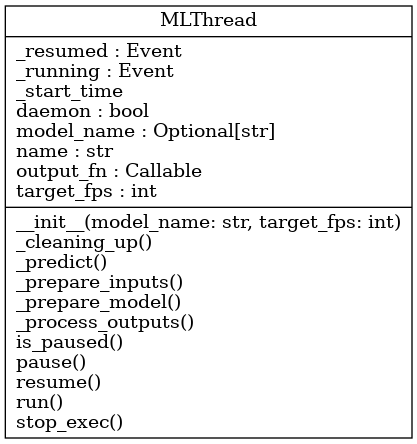
\includegraphics[scale=0.5]{images/chapter5/mlthread_uml.png}
	\caption{UML διάγραμμα της κλάσης \texttt{MLThread}.}
	\label{fig:mlthread}
\end{figure}

\noindent\textbf{Περιγραφή Κλάσης}

Η κλάση \texttt{MLThread} είναι μία αφαιρετική κλάση διαχείρισης ενός thread μοντέλου μηχανικής μάθησης. Κληρονομώντας από την \texttt{threading.Thread}\footnote{\href{https://docs.python.org/3/library/threading.html\#threading.Thread}{https://docs.python.org/3/library/threading.html\#threading.Thread}} παρέχει απαραίτητες μεθόδους για την έναρξη, σταματημό ή παύση του thread. Με την αρχικοποίηση του thread μπαίνει στον βρόγχο λειτουργίας του στην μέθοδο \texttt{run()} η οποία σε μία επανάληψη, εκτελεί μία εκτίμηση του μοντέλου. Επιπλέον, η κλάση \texttt{MLThread} υλοποιεί το σχεδιαστικό πρότυπο \textsl{Template design pattern}\footnote{\href{https://en.wikipedia.org/wiki/Template\_method\_pattern}{https://en.wikipedia.org/wiki/Template\_method\_pattern}} κατά το οποίο ορίζονται η αλληλουχία των βημάτων του αλγορίθμου και στην συνέχεια οι κλάσεις που την κληρονομούν είναι υπεύθυνες για την υλοποίηση αυτών καθ'αυτών των βημάτων.

\noindent\textbf{Χαρακτηριστικά κλάσης}
\begin{itemize}
	\item \texttt{\_resumed}: \texttt{threading.Event}\footnote{\href{https://docs.python.org/3/library/threading.html\#event-objects}{https://docs.python.org/3/library/threading.html\#event-objects}. Συνοπτικά, μπορούμε να φανταστούμε την κλάση αυτή ως μια boolean μεταβλητή, την οποία μπορεί το thread να περιμένει μέχρι να γίνει true.} που καθορίζει αν ο βρόγχος λειτουργίας του thread λειτουργεί ή είναι σε παύση.
	\item \texttt{\_running}: \texttt{threading.Event} το οποίο αρχικοποιείται με \texttt{set} και όσο παραμένει ο βρόγχος λειτουργίας συνεχίζεται. Όταν γίνει \texttt{clear} το thread τερματίζει την μέθοδο \texttt{run} του.
	\item \texttt{\_start\_time}: Η χρονική στιγμή στην αρχή της επανάληψης του βρόγχου λειτουργίας.
	\item \texttt{daemon}: Μεταβλητή που καθορίζει αν το thread τρέχει σαν daemon. Ορίζεται ως true ώστε όταν τερματίσει το main thread να τερματίσει και αυτό.
	\item \texttt{model\_name}: Το όνομα του μοντέλου μηχανικής μάθησης.
	\item \texttt{name}: Το όνομα του thread.
	\item \texttt{output\_fn}: Η μέθοδος που καλείται με όρισμα τα αποτελέσματα του μοντέλου.
	\item \texttt{target\_fps}: Οι μέγιστες προβλέψεις ανά δευτερόλεπτο που επιτρέπεται να λειτουργήσει το μοντέλο.
\end{itemize}

\noindent\textbf{Μέθοδοι Κλάσης}
Οι μέθοδοι \texttt{\_prepare\_models}, \texttt{\_prepare\_inputs}, \texttt{\_predict}, \texttt{\_process\_outputs} και \texttt{\_cleaning\_up} είναι αφηρημένες (abstract) και πρέπει να υλοποιηθούν από τους κληρονόμους της κλάσης \texttt{MLThread}.

\begin{itemize}
	\item \texttt{\_\_init\_\_(model\_name, target\_fps)}: Καθορίζει το όνομα του thread με βάση το όνομα του μοντέλου \texttt{model\_name}. Επίσης, καλεί την μέθοδο \texttt{start()} της κλάσης \texttt{threading.Thread}, η οποία ξεκινάει το thread, τρέχοντας την μέθοδο \texttt{run()}. Το thread ξεκινάει την λειτουργία του στην αρχικοποίηση του ώστε να αρχίσουν να φορτώνουν απευθείας τα μοντέλα μηχανικής μάθησης, ξεκινώντας όμως σε κατάσταση παύσης.
	\item \texttt{is\_paused()}: Επιστρέφει true αν το thread βρίσκεται σε κατάσταση παύσης και false διαφορετικά.
	\item \texttt{pause()}: Κάνει \texttt{clear} το \texttt{\_resumed}, οπότε το thread κάνει παύση στην εκτέλεση του βρόγχου λειτουργίας του.
	\item \texttt{resume()}: Κάνει \texttt{set} το \texttt{\_resumed}, οπότε το thread συνεχίζει την εκτέλεση του βρόγχου λειτουργίας.
	\item \texttt{stop\_exec()}: Κάνει \texttt{clear} το \texttt{\_running}, οπότε το thread τερματίζει τον βρόγχο λειτουργίας του.
	\item \texttt{run()}: Αρχικά, φορτώνει το μοντέλο μηχανικής μάθησης εκτελώντας την μέθοδο \texttt{\_prepare\_model()}. Έπειτα, ξεκινάει ο κύριος βρόγχος λειτουργίας του thread που τρέχει όσο το \texttt{\_running} είναι \texttt{set}. Στην αρχή του βρόγχου, αναμένεται μέχρι το \texttt{\_resumed} να γίνει \texttt{set}. Τότε, θέτετε το \texttt{\_start\_time}, ετοιμάζονται οι είσοδοι του μοντέλου, εκτελώντας την \texttt{\_prepare\_inputs()}. Οι είσοδοι δίνονται ως όρισμα στην \texttt{\_predit()} και στη συνέχεια τα αποτελέσματα στην \texttt{\_process\_outputs}. Τέλος, αν ο χρόνος που έγινε η εκτίμηση είναι πιο γρήγορος από τον μέγιστο χρόνο ώστε να μην ξεπερνιούνται τα \texttt{\_target\_fps}, το thread κοιμάται, εκτελώντας την \texttt{time.sleep()}. Με το πέρας του βρόγχου λειτουργίας, εκτελείται η \texttt{\_cleaning\_up()} για να κλείσουν ενδεχόμενα ανοιχτά resources. 
\end{itemize}

\newpage
\subsubsection{HMRThread}
\label{sec:hmr_thread}

\begin{figure}[H]
	\centering
	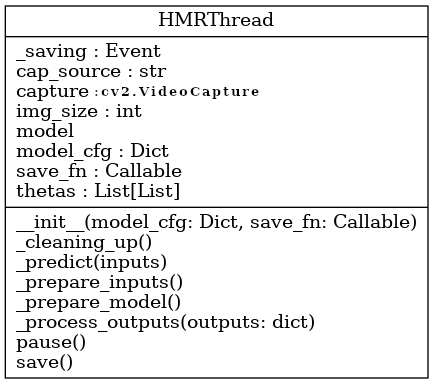
\includegraphics[scale=0.5]{images/chapter5/hmr_thread_uml.png}
	\caption{UML διάγραμμα της κλάσης \texttt{HMRThread}.}
	\label{fig:hmrthread}
\end{figure}

\noindent\textbf{Περιγραφή Κλάσης}

Η κλάση \texttt{HMRThread} είναι το thread που ελέγχει το μοντέλο μηχανικής μάθησης HMR, διεκπεραιώνοντας έτσι τις εκτιμήσεις πόζας. Σε κάθε επανάληψη του βρόγχου λειτουργίας του δέχεται ως είσοδο ένα καρέ από την κάμερα του χρήστη ή από ένα βίντεο και παράγει τις 85 παραμέτρους SMPL, τις 3D συντεταγμένες των 6980 κορυφών πλέγματος και 24 σημείων κλειδιών του ανθρώπινου σώματος.

\noindent\textbf{Χαρακτηριστικά κλάσης}
\begin{itemize}
	\item \texttt{\_saving}: \texttt{threading.Event} που καθορίζει αν θα αποθηκευτούν οι 82\footnote{Οι 3 παράμετροι που παραλείπονται κατά την αποθήκευση είναι οι 3 συντεταγμένες της θέσης της κάμερας} παράμετροι SMPL, για χρήση ως δεδομένων άσκησης αναφοράς, ή όχι.
	\item \texttt{cap\_source}: Καθορίζει την πηγή λήψης των καρέ. Παίρνει την τιμή \textsl{"cam"}, οπότε η πηγή είναι η κάμερα του χρήστη, ενώ διαφορετικά παίρνει την τιμή του path σε ένα αρχείο βίντεο.
	\item \texttt{capture}: Με βάση την τιμή του \texttt{cap\_source} αρχικοποιείται η \texttt{capture}, κλάσης \texttt{VideoCapture}\footnote{\href{https://docs.opencv.org/3.4/d8/dfe/classcv\_1\_1VideoCapture.html}{https://docs.opencv.org/3.4/d8/dfe/classcv\_1\_1VideoCapture.html}} της \texttt{OpenCV}, μέσω της οποίας γίνεται η λήψη του καρέ.
	\item \texttt{img\_size}: Η διάσταση της τετραγωνικής εικόνας που δέχεται το μοντέλο. Στην συγκεκριμένη υλοποίηση αυτή είναι $224 \times 224$.
	\item \texttt{model}: Το μοντέλο HMR, κλάσης \texttt{HMR}, αφού φορτωθεί στην μνήμη.
	\item \texttt{model\_config}: Ένα namespace με μεταβλητές που καθορίζουν τον τρόπο λειτουργίας του μοντέλου HMR. Περιλαμβάνει τις διαστάσεις τις εικόνας, τον αριθμό σταδίων του επαναληπτικού παλινδρομητή (όπως περιγράφηκε στην \ref{sec:hmr}), τα paths των αρχείων των προ-εκπαιδευμένων μοντέλων και τον αριθμό των σημείων κλειδιών.
	\item \texttt{save\_fn}: Η συνάρτηση που πρέπει να κληθεί για την αποθήκευση των παραμέτρων.
	\item \texttt{thetas}: Οι 82 παράμετροι SMPL που πρέπει να αποθηκευτούν για κάθε καρέ.
\end{itemize}

\noindent\textbf{Μέθοδοι Κλάσης}

\begin{itemize}
	\item \texttt{\_prepare\_model()}: Αρχικοποιεί το \texttt{session}\footnote{\href{https://www.tensorflow.org/api\_docs/python/tf/compat/v1/Session}{https://www.tensorflow.org/api\_docs/python/tf/compat/v1/Session}} και το \texttt{graph}\footnote{\href{https://www.tensorflow.org/api\_docs/python/tf/Graph}{https://www.tensorflow.org/api\_docs/python/tf/Graph}} του Tensorflow, φορτώνει το μοντέλο και αποθηκεύει χρησιμοποιώντας την συνάρτηση \texttt{summary.FileWriter()} του Tensorflow τον γράφο του μοντέλου, για οπτικοποίηση με το Tensorboard.
	\item \texttt{\_prepare\_inputs()}: Λαμβάνει ένα καρέ από την πηγή, καλώντας την συνάρτηση \texttt{read()} του \texttt{VideoCapture}. Έπειτα, το προεπεξεργάζεται, σμικρύνοντας την εικόνα στις διαστάσεις \texttt{image\_size}, διατηρώντας όμως τις αναλογίες διαστάσεων. Επιστρέφει την εικόνα καρέ και μία boolean δηλώντας αν ήταν εφικτή η απόκτηση του καρέ. Για την αποσφαλμάτωση, χρησιμοποιείται η συνάρτηση \texttt{imshow} της \texttt{OpenCV} για την προβολή των εικόνων καρέ σε ένα άλλο παράθυρο.
	\item \texttt{\_predict(inputs)}: Αν η εικόνα είχε ληφθεί με επιτυχία, καλεί την μέθοδο \texttt{predict()} του μοντέλου HMR για την εκτίμηση πόζας και επιστρέφει τις συντεταγμένες των κορυφών και των σημείων κλειδιών. Αν η \texttt{\_saving} είναι \textsl{set} τότε όσο έρχονται επιτυχώς καρέ, αποθηκεύονται στην \texttt{thetas}, ενώ όταν δεν έρθει εικόνα γίνεται παύση του thread, καλώντας την \texttt{pause()} και επιστρέφονται τα \texttt{thetas}.
	\item \texttt{\_process\_outputs(outputs)}: Αν υπάρχουν τα \texttt{thetas} στο όρισμα \texttt{outputs} τότε απλά καλείται η \texttt{save\_fn()} για αποθήκευση των παραμέτρων. Διαφορετικά, καλείται η \texttt{output\_fn()} με όρισμα τις κορυφές και τα σημεία κλειδιά.
	\item \texttt{\_cleaning\_up}: Απελευθερώνει το \texttt{capture}, δηλαδή την κάμερα ή το αρχείο βίντεο, και κλείνει όλα τα παράθυρα που άνοιξαν μέσω του \texttt{OpenCV}.
	\item \texttt{save()}: Επαναφέρει τα \texttt{thetas} σε κενή λίστα και κάνει \textsl{set} την \texttt{\_saving}.
\end{itemize}


\newpage
\subsubsection{SMPLThread}
\label{sec:smpl_thread}

\begin{figure}[H]
	\centering
	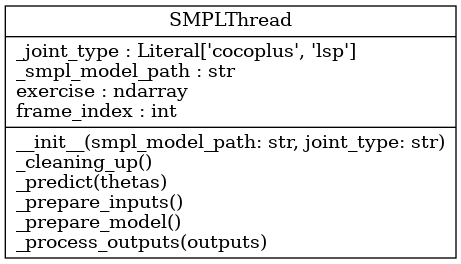
\includegraphics[scale=0.5]{images/chapter5/smpl_thread_uml.png}
	\caption{UML διάγραμμα της κλάσης \texttt{SMPLThread}.}
	\label{fig:smplthread}
\end{figure}

\noindent\textbf{Περιγραφή Κλάσης}

Η κλάση \texttt{SMPLThread} είναι το thread που ελέγχει το μοντέλο μηχανικής μάθησης SMPL, διεκπεραιώνοντας την μετατροπή των 82 παραμέτρων SMPL στις 3D συντεταγμένες των 6980 κορυφών πλέγματος και των 24 σημείων κλειδιών του ανθρώπινου σώματος, όπως αναλύθηκαν στο \ref{sec:smpl}. Τοιουτοτρόπως, σε κάθε επανάληψη του βρόγχου λειτουργίας του \texttt{SMPLThread} γίνεται ακριβώς αυτή η μετατροπή.

\noindent\textbf{Χαρακτηριστικά κλάσης}
\begin{itemize}
	\item \texttt{\_joint\_type}: Ανάλογα με την τιμή του επιστρέφονται τα 19 σημεία κλειδιά ορισμένα με την σειρά του προτύπου \textsl{coco}\footnote{\href{https://cocodataset.org/}{https://cocodataset.org/}} ή τα 14 του \textsl{lsp}\footnote{\href{https://dbcollection.readthedocs.io/en/latest/datasets/leeds\_sports\_pose\_extended.html}{https://dbcollection.readthedocs.io/en/latest/datasets/leeds\_sports\_pose\_extended.html}} dataset. Εντούτοις, στην εφαρμογή χρησιμοποιούνται τα 24 σημεία κλειδιά με την σειρά ορισμένη από το SMPL\footnote{Για το πλήρες κινηματικό δέντρο, σελίδα 24 του pdf \href{https://files.is.tue.mpg.de/black/talks/SMPL-made-simple-FAQs.pdf}{https://files.is.tue.mpg.de/black/talks/SMPL-made-simple-FAQs.pdf}}.
	\item \texttt{smpl\_model\_path}: To path του προ-εκπαιδευμένου μοντέλου SMPL.
	\item \texttt{exercise}: Οι 82 παράμετροι SMPL για κάθε καρέ της άσκησης προς αναπαραγωγή.
	\item \texttt{frame\_index}: Ο δείκτης καρέ που καθορίζει το σημείο της αναπαραγωγής. Μεταβάλλοντας αυτό το χαρακτηριστικό ελέγχεται η αναπαραγωγή.
\end{itemize}

\noindent\textbf{Μέθοδοι Κλάσης}

\begin{itemize}
	\item \texttt{\_prepare\_model()}: Αρχικοποιεί το \texttt{session} και το \texttt{graph} του Tensorflow και χτίζει τον υπολογιστικό γράφο του μοντέλου. Προς επίτευξη αυτού του σκοπού, ορίζονται οι 82 παράμετροι ως tensors εισόδου και οι κορυφές και τα σημεία κλειδιά ως tensors εξόδου και καλείται η συνάρτηση μετατροπής του SMPL.
	\item \texttt{\_prepare\_inputs()}: Λαμβάνει από την \texttt{exercise} τις παραμέτρους SMPL ανάλογα με το τωρινό \texttt{frame\_index} και τις επιστρέφει.
	\item \texttt{\_predict(inputs)}: Καλείται η συνάρτηση \texttt{run()} του \texttt{session} ώστε να γίνει η εκτίμηση των κορυφών και των σημείων κλειδιών, τα οποία επιστρέφονται.
	\item \texttt{\_process\_outputs(outputs)}: Καλείται η συνάρτηση \texttt{output\_fn()} με ορίσματα τις εξόδους του SMPL καθώς και πληροφορίες για το καρέ, δηλαδή τον δείκτη \texttt{frame\_index} και την στιγμή λήψης του καρέ, \texttt{\_start\_time}.
	\item \texttt{\_cleaning\_up}: Δεν υλοποιεί κάποια λειτουργία.
\end{itemize}

\newpage

\subsection{Renderer}
\label{sec:renderer}

\begin{figure}[H]
	\centering
	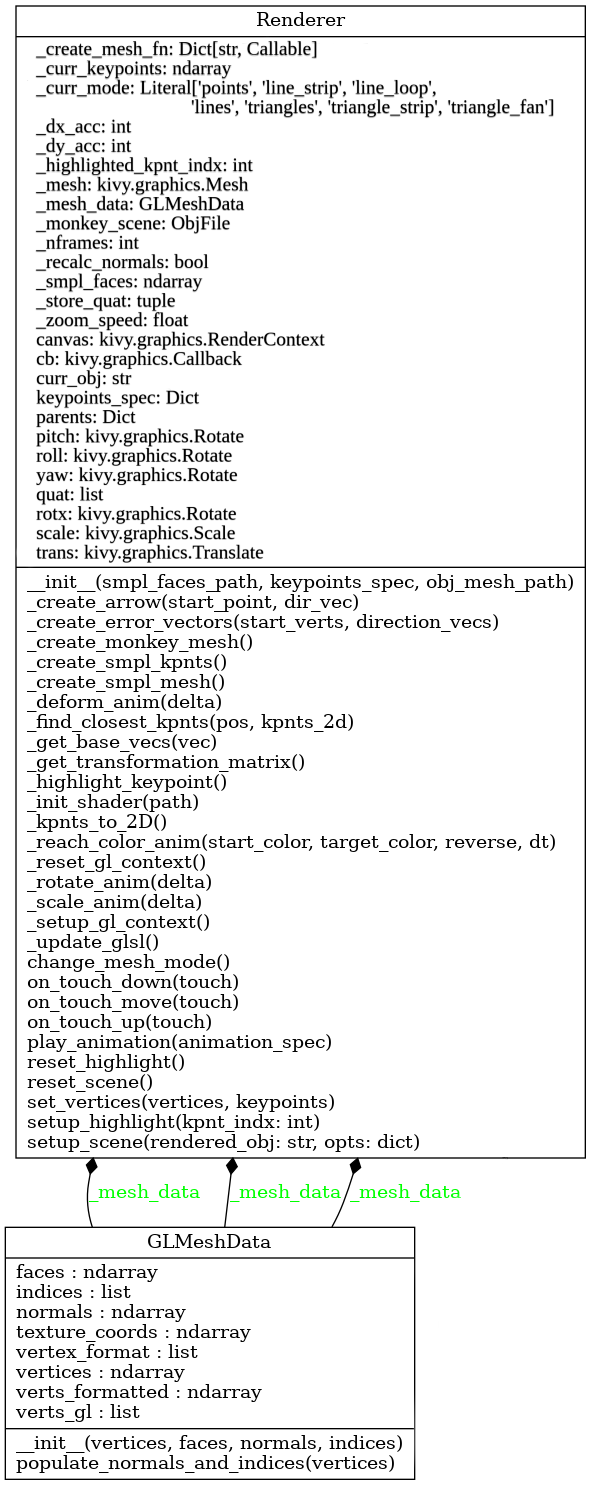
\includegraphics[scale=0.4]{images/chapter5/renderer_uml.png}
	\caption{UML διάγραμμα της κλάσης \texttt{Renderer} και των σχέσεων της.}
	\label{fig:renderer_uml}
\end{figure}

\noindent\textbf{Περιγραφή Κλάσης}

Η κλάση \texttt{Renderer} είναι η κλάση που ελέγχει την απεικόνιση του ανθρώπινου πλέγματος, του σκελετού αλλά και των διορθωτικών βελών. Επιπλέον, παρέχει τη δυνατότητα αναπαραγωγής απλών εφέ πάνω στο πλέγμα, περιστροφής του πλέγματος με μονό κρατημένο κλικ, τη μεγέθυνση ή σμίκρυνση του πλέγματος με χρήση της ροδέλας του ποντικιού και κατά την λειτουργία \textsl{επιμελητή} την αλλαγή του χρώματος στην περιοχή ενός σημείου κλειδιού με μονό κλικ ώστε να καθιστά εμφανές το διαλεγμένο σημείο κλειδί προς επεξεργασία (θα αναφερόμαστε σε αυτή την λειτουργία ως \textsl{highlight}).

Έτσι, ο \texttt{Renderer} για τον καθορισμό των δεδομένων των αντικειμένων στην σκηνή χρησιμοποιεί την κλάση \texttt{GLMeshData} και για την απεικόνιση αυτών χρησιμοποιείται το χαμηλότερου επιπέδου API της \textsl{OpenGL ES 2.0} μέσω των bindings στην Kivy και συγκεκριμένα του πακέτου \texttt{kivy.graphics}\footnote{\href{https://kivy.org/doc/stable/api-kivy.graphics.html}{https://kivy.org/doc/stable/api-kivy.graphics.html}}.

Πιο συγκεκριμένα, οι κορυφές αποθηκεύονται στην κλάση \texttt{GLMeshData} η οποία μέσω του χαρακτηριστικού \texttt{faces}, ενός πίνακα $F \times 3$, καθορίζει ποιες 3 κορυφές σχηματίζουν κάθε ένα από τα F τρίγωνα που απαρτίζουν το ανθρώπινο πλέγμα. Ταυτόχρονα, μέσω της συνάρτησης \texttt{populate\_normals\_and\_indices()} υπολογίζει τα normals για κάθε κορυφή. Τέλος, η OpenGL για την είσοδο των κορυφών απαιτεί όλες τις κορυφές, \texttt{vertices}, τα normals τους, \texttt{normals}, και τις UV συντεταγμένες για καθορισμό texture, \texttt{texture\_coords}, να διατάσσονται σε μία μονοδιάστατη λίστα \texttt{verts\_gl} με συγκεκριμένη σειρά στην οποία αναφέρεται η λίστα \texttt{indices} για τον καθορισμό των τριγώνων.

\noindent\textbf{Χαρακτηριστικά κλάσης}
\begin{itemize}
	\item \texttt{\_create\_mesh\_fn}: Ένα dictionary με keys το όνομα ενός αντικειμένου και values την μέθοδο της κλάσης η οποία το κατασκευάζει.
	\item \texttt{\_curr\_keypoints}: Τα σημεία κλειδιά σε ένα συγκεκριμένο καρέ. Χρησιμοποιείται για να ορίζεται το κέντρο του highlight δυναμικά καθώς αλλάζει η πόζα του ανθρώπου.
	\item \texttt{\_curr\_mode}: Ο τρόπος με τον οποίο βάφονται οι κορυφές. Η επιλογή\textsl{triangles} είναι ο συνηθισμένος τρόπος όπου βάφεται η εξωτερική όψη του κάθε τριγώνου.
	\item \texttt{\_dx\_acc \& \_dy\_acc}: Συσσωρευτές μετακίνησης του ποντικιού στους άξονες της οθόνης x και y αντίστοιχα από την στιγμή που έγινε το πρώτο κλικ. Χρησιμοποιούνται για την ομαλή περιστροφή του αντικειμένου.
	\item \texttt{\_highlighted\_kpnt\_indx}: Ο δείκτης του επιλεγμένου σημείου κλειδιού κατά την επεξεργασία του στην λειτουργία \textsl{επιμελητή}.
	\item \texttt{\_mesh}: Το πλέγμα του αντικειμένου της σκηνής, κλάσης \texttt{kivy.graphics.Mesh}\footnote{\href{https://kivy.org/doc/stable/api-kivy.graphics.html\#kivy.graphics.Mesh}{https://kivy.org/doc/stable/api-kivy.graphics.html\#kivy.graphics.Mesh}}.
	\item \texttt{\_mesh\_data}: Τα δεδομένα κορυφών, normals και δεικτών (indices) που δίνονται σαν όρισμα στην κατασκευή του \texttt{\_mesh}.
	\item \texttt{\_monkey\_scene}: Το αντικείμενο τύπου \texttt{.obj} προς απεικόνιση για αποσφαλμάτωση.
	\item \texttt{\_nframes}: Ο αριθμός των καρέ που έχουν απεικονιστεί από την αρχικοποίηση αυτής της σκηνής.
	\item \texttt{\_recalc\_normals}: Καθορίζει αν πρέπει να υπολογιστούν τα normals. Ο υπολογισμός των normals γίνεται μόνο όταν αρχικοποιηθεί η σκηνή. Αυτό δημιουργεί προβλήματα στον τρόπο που φωτίζεται το ανθρώπινο πλέγμα, αλλά ο υπολογισμός γίνεται στην CPU απαιτώντας υπολογιστική ισχύ και μειώνοντας τον αριθμό καρέ ανά δευτερόλεπτο.
	\item \texttt{\_smpl\_faces}: Πίνακας $F \times 3$ όπου καθορίζονται οι 3 κορυφές των F τριγώνων που απαρτίζουν το ανθρώπινο πλέγμα.
	\item \texttt{\_store\_quat}: To αρχικό τετραδόνιο της περιστροφής του αντικειμένου. Χρησιμοποιείται για την ομαλή περιστροφή στο διαρκές κλικ.
	\item \texttt{\_zoom\_speed}: Η ταχύτητα με την οποία γίνεται μεγέθυνση ή σμίκρυνση του αντικειμένου με την ροδέλα.
	\item \texttt{canvas}: Ο καμβάς πάνω στον οποίο γίνεται η απεικόνιση. 
	\item \texttt{cb}: Μέθοδος που καλείται όταν γίνεται η διαδικασία της παραγωγής γραφικών πάνω στον καμβά.
	\item \texttt{curr\_obj}: Το όνομα του αντικειμένου που απεικονίζει ο \texttt{Renderer}.
	\item \texttt{keypoints\_spec}: Ο προσδιορισμός των χαρακτηριστικών των σημείων κλειδιών.
	\item \texttt{parents}: Το κινηματικό δέντρο των σημείων κλειδιών του μοντέλου SMPL.
	\item \texttt{roll \& pitch \& yaw}: Η περιστροφή του αντικειμένου γύρω από τους άξονες σχετικά με τον προσανατολισμό του.
	\item \texttt{quat}: Το τετραδόνιο της περιστροφής του αντικειμένου καθώς περιστρέφεται με το διαρκές κλικ. Χρησιμοποιείται για την ομαλή περιστροφή του αντικειμένου.
	\item \texttt{rotx}: Η περιστροφή του αντικειμένου γύρω από τον άξονα x.
	\item \texttt{scale}: Η μεγέθυνση ή σμίκρυνση του αντικειμένου.
	\item \texttt{trans}: Η μετατόπιση του αντικειμένου.
\end{itemize}

\noindent\textbf{Μέθοδοι Κλάσης}

\begin{itemize}
	\item \texttt{\_\_init\_\_(smpl\_faces\_path, keypoints\_spec, obj\_mesh\_path)}: Υπολογίζεται το κινηματικό δέντρο, τo \texttt{parents}, με βάση το \texttt{keypoint\_spec}, αρχικοποιείται ο καμβάς \texttt{canvas}, φορτώνονται οι shaders με κλήση της \texttt{\_init\_shader()}, μηδενίζονται τα χαρακτηριστικά \texttt{\_store\_quat}, \texttt{\_dx\_acc}, \texttt{\_dy\_acc}, \texttt{\_nframes}, \texttt{curr\_obj} και παίρνει την τιμή \textsl{triangles} η \texttt{\_curr\_mode}.
	
	\item \texttt{\_create\_arrow(start\_point, dir\_vec)}: Δημιουργεί ένα πλέγμα βέλους που ξεκινάει από το σημείο \texttt{start\_point} και δείχνει προς την κατεύθυνση του διανύσματος \texttt{dir\_vec}.
	\item \texttt{\_create\_error\_vectors(start\_verts, direction\_vecs)}: Για κάθε σημείο στη λίστα \texttt{start\_verts} και κατεύθυνση του \texttt{start\_verts}, δημιουργεί ένα βέλος. Όλα τα βέλη υφίστανται μία περιστροφή 180 μοιρών γύρω από τον άξονα x, με χρήση του \texttt{rotx}, επειδή οι άξονες x και y του SMPL και του καμβά είναι αντιστραμμένη. Επίσης, μετατοπίζει τα βέλη κατά τον άξονα z, με χρήση του \texttt{trans}, ώστε να φαίνονται πιο έντονα και καθαρά στην απεικόνιση.
	
	\item \texttt{create\_monkey\_mesh() \& \_create\_smpl\_mesh() \& \_create\_smpl\_kpnts()}: Οι μέθοδοι δημιουργίας των αντικειμένων 'monkey', 'smpl mesh' και 'smpl skeleton' αντίστοιχα. Προσαρμόζουν τα δεδομένα κορυφών στην επιθυμητή μορφή με χρήση της κλάσης \texttt{GLMeshData}. Οι μέθοδοι του μοντέλου SMPL εφαρμόζουν επίσης μία περιστροφή 180 μοιρών γύρω από τον άξονα x.
	
	\item \texttt{\_deform\_anim(delta)}: Εφαρμόζει μία τυχαία μικρή μετατόπιση όλων των κορυφών του πλέγματος προς τυχαίες διευθύνσεις.
	
	\item \texttt{\_find\_closest\_kpnts(pos, kpnts\_2d)}: Βρίσκει το πιο κοντινό σημείο κλειδί στην θέση της οθόνης \texttt{pos} από την λίστα με τις 2D συντεταγμένες όλων των σημείων κλειδιών \texttt{kpnts\_2d}, και επιστρέφει το όνομα του.
	
	\item \texttt{\_get\_base\_vecs(vec)}: Με δεδομένο ένα διάνυσμα \texttt{vec} βρίσκει άλλα δύο διανύσματα με τα οποία δημιουργούνε μία βάση ορθοκανονικού συστήματος, και τα επιστρέφει.
	
	\item \texttt{\_get\_transformation\_matrix()}: Υπολογίζει τον πίνακα γραμμικού μετασχηματισμού βάση όλων των περιστροφών, μετατοπίσεων και μεγεθύνσεων που έχουν γίνει.
	
	\item \texttt{\_highlight\_keypoint()}: Αν υπάρχει η \texttt{\_highlighted\_kpnt\_indx}, δηλαδή κάποιο σημείο κλειδί είναι επιλεγμένο, τότε θέτει τις μεταβλητές κέντρου σφαίρας \texttt{canvas['sphere\_center']} στο σημείο αυτό και ακτίνας \texttt{canvas['sphere\_radius']}, που καθορίζεται από το \texttt{keypoints\_spec}, τις οποίες μεταβλητές διαβάζει ο shader. Έτσι, στον shader σχηματίζεται μία σφαίρα και όσες κορυφές βρίσκονται εντός της χρωματίζονται διαφορετικά δημιουργώντας το highlight εφέ.
	
	\item \texttt{\_kpnts\_to\_2D()}: Με βάση των πίνακα Μετασχηματισμού-Κάμερας (modelview) και τον πίνακα Προβολής (projection) καθώς και τον πίνακα μετασχηματισμών (transformation) υπολογίζονται η 2D συντεταγμένες των σημείων κλειδιών σε αυτό το καρέ απεικόνισης.
	
	\item \texttt{\_reach\_color\_anim(start\_color, target\_color, reverse, dt)}: Παίζει ένα εφέ στο απεικονιζόμενο αντικείμενο. Το αντικείμενο ξεκινάει από το RGB χρώμα \texttt{start\_color}, φτάνει με γραμμική παρεμβολή στο χρώμα \texttt{target\_color}, και αν η \texttt{reverse} είναι true επιστρέφει ξανά στο αρχικό χρώμα με πιο αργό ρυθμό.
	
	\item \texttt{\_setup\_gl\_context() \& \_reset\_gl\_context()}: Μέθοδοι που χρησιμοποιούνται ως \texttt{kivy.graphics.Callback} για να θέσουν και να επαναφέρουν αντίστοιχα το περιβάλλον δημιουργίας γραφικών στον καμβά.
	
	\item \texttt{\_update\_glsl()}: Θέτει το επίπεδο αποκοπής καθορίζοντας τον πίνακα προβολής.
	
	\item \texttt{\_rotate\_anim(delta)}: Παίζει ένα εφέ όπου το αντικείμενο περιστρέφεται συνεχόμενα γύρω από τον κατακόρυφο άξονα y.
	
	\item \texttt{\_scale\_anim(delta)}: Παίζει ένα εφέ όπου το αντικείμενο μεγεθύνεται και σμικρύνεται ταυτόχρονα στους άξονες x και y ακολουθώντας δύο ημιτονοειδής συναρτήσεις με διαφορά φάσης 180 μοίρες.
	
	\item \texttt{on\_touch\_down(touch)}: Αν υπάρχει απεικονιζόμενο πλέγμα και το κλικ έγινε στην περιοχή του widget, τότε αν το γεγονός προκλήθηκε από την ροδέλα σμικρύνεται ή μεγεθύνεται το αντικείμενο. Διαφορετικά, μηδενίζονται οι συσσωρευτές \texttt{\_dx\_acc} και \texttt{\_dy\_acc}, αποθηκεύεται το αρχικό τετραδόνιο περιστροφής στην \texttt{\_store\_quat} και δεσμεύεται το γεγονός του κλικ από το widget.
	
	\item \texttt{on\_touch\_move(touch)}: Αν το κλικ είναι δεσμευμένο από το widget του \texttt{Renderer}, τότε αυξάνονται οι \texttt{\_dx\_acc} και \texttt{\_dy\_acc} ανάλογα με την μετατόπιση του κλικ, μετατρέπονται οι μετατοπίσεις σε τετραδόνιο το οποίο πολλαπλασιάζεται με το αρχικό \texttt{\_store\_quat} παράγοντας το τετραδόνιο περιστροφής \texttt{quat}. Τέλος, το \texttt{quat} μετατρέπεται πάλι σε γωνίες και έτσι καθορίζεται η περιστροφή στα \texttt{roll, pitch} και \texttt{yaw}.
	
	\item \texttt{on\_touch\_up(touch)}: Όταν απελευθερωθεί το κλικ, αν δεν είχε κουνηθεί καθόλου και δεν ήταν η ροδέλα, τότε διαχειρίζεται το μονό κλικ, υπολογίζοντας το κοντινότερο σημείο κλειδί, με χρήστη των \texttt{\_kpnts\_to\_2D()} και \texttt{\_find\_closest\_kpnts()}, και εκτελώντας την \texttt{single\_click\_handle()} αν έχει ορισθεί από το action που διαχειρίζεται αυτόν τον \texttt{Renderer}.
	
	\item \texttt{play\_animation(animation\_spec)}: Με βάση το όνομα ενός εφέ, \texttt{animation\_spec}, παίζει το αντίστοιχο εφέ.
	
	\item \texttt{reset\_highlight()}: Αν υπάρχει το \texttt{\_highlighted\_kpnt\_indx}, το διαγράφει και θέτει την ακτίνα της σφαίρας, \texttt{canvas['sphere\_radius']}, στο 0.
	
	\item \texttt{reset\_scene()}: Καθαρίζει τον καμβά από όλα τα πλέγματα αντικειμένων και μηδενίζει την \texttt{\_nframes}.
	
	\item \texttt{set\_vertices(vertices, keypoints)}: Αν το απεικονιζόμενο αντικείμενο είναι το \textsl{smpl\_mesh} ή το \textsl{smpl\_kpnts} Θέτει τις κορυφές του \texttt{GLMeshData} να είναι τα \texttt{vertices} ή \texttt{keypoints} αντίστοιχα. Επίσης, αυξάνει τον μετρητή καρέ, \texttt{\_nframes}, κατά ένα και αφού θέσει τα καινούργια σημεία κλειδιά στην \texttt{\_curr\_keypoints} καλεί την \texttt{\_highlight\_keypoint()}.
	
	\item \texttt{setup\_scene(rendered\_obj, opts)}: Θέτει την \texttt{\_recalc\_normals} σε true, προετοιμάζει τον καμβά για απεικόνιση με OpenGL, καλώντας τις \texttt{\_setup\_gl\_context} και στο πέρας της απεικόνισης την \texttt{\_reset\_gl\_context}, θέτει τις αρχικές τιμές των περιστροφών, μετατοπίσεων και μεγεθύνσεων, καλεί κάποια συνάρτηση δημιουργίας πλέγματος αντικειμένου με βάση το όνομα του αντικειμένου προς απεικόνιση \texttt{rendered\_object} και την αντιστοιχία \texttt{\_create\_mesh\_fn}.
	
	
\end{itemize}
